\documentclass{report}

% Packages for math symbols and equations
\usepackage[T1]{fontenc}
\usepackage[utf8]{inputenc}

\usepackage[margin=1.4in]{geometry}
\usepackage{graphicx}

\usepackage{amssymb,amsthm, amsmath}
%\usepackage{mathtools}
%\numberwithin{equation}{section}

\usepackage[
natbib,
style=alphabetic,
maxbibnames=10,  
sorting=ydnt,
url=false,
doi=false,
sortcites,
defernumbers,
backref,
backend=biber
]{biblatex}
\addbibresource{bibliography.bib}

\usepackage{hyperref}

\usepackage{todonotes}
%\setuptodonotes{inline}
\usepackage{url}

\usepackage[nameinlink, capitalise, noabbrev]{cleveref}

\usepackage{xfrac}
\usepackage{nicefrac}

\usepackage{soul}

\usepackage{bbm}

\usepackage{enumitem}

%For double brackets \llbracket \rrbracket
\usepackage{stmaryrd}

\crefname{assumption}{Assumption}{Assumptions}

\newtheorem{theorem}{Theorem}

\newtheorem{proposition}{Proposition}[section]
\newtheorem{lemma}{Lemma}[section]
\newtheorem{corollary}{Corollary}[section]
\theoremstyle{remark}
\newtheorem{remark}{Remark}[section]


\theoremstyle{definition}
\newtheorem{example}{Example}[section]
\newtheorem{counterexample}{Counterexample}[section]
\newtheorem{definition}{Definition}[section]
\newtheorem{assumption}{Assumption}

%\numberwithin{equation}{section}

%\renewcommand{\baselinestretch}{2}

%\newcounter{hypcounter}

\newcommand{\N}{\mathbb{N}}
\newcommand{\Z}{\mathbb{Z}}
\newcommand{\R}{\mathbb{R}}
%\DeclareMathOperator{\dom}{dom}
\newcommand{\closure}[1]{\overline{#1}}
\newcommand{\norm}[1]{\left\Vert #1 \right\Vert}
\newcommand{\seminorm}[1]{\left[ #1 \right]}
\newcommand{\abs}[1]{\left\vert #1 \right\vert}
%\DeclareMathOperator{\divtmp}{div}
\renewcommand{\div}{\divtmp}
% \DeclareMathOperator{\argmin}{arg\,min}
% \DeclareMathOperator{\argmax}{arg\,max}
% \DeclareMathOperator{\esssup}{ess\,sup}
% \DeclareMathOperator{\essinf}{ess\,inf}
\renewcommand{\st}{\,:\,}
% \DeclareMathOperator{\supp}{supp}
\newcommand{\dx}{\,\mathrm{d}x}
\renewcommand{\d}{\,\mathrm{d}}
\newcommand{\dH}{\,\mathrm{d}\mathcal{H}^{n-1}(x)}
% \DeclareMathOperator{\sign}{sign}
\newcommand{\eps}{\varepsilon}
% \DeclareMathOperator{\dist}{dist}
% \DeclareMathOperator{\Lip}{Lip}
\newcommand{\KR}{\mathrm{KR}}
\newcommand{\C}{\mathrm{C}}
\renewcommand{\L}{\mathrm{L}}
\newcommand{\W}{\mathrm{W}}
\newcommand{\M}{\mathcal M}
\newcommand{\grad}{\nabla}
\newcommand{\hess}{\mathrm{D}^2}
\newcommand{\defeq}{:=}
% \DeclareMathOperator{\diam}{diam}
\newcommand{\Set}[1]{\left\lbrace#1\right\rbrace}
\newcommand{\scale}{\eps}
\newcommand{\res}{\delta}


\newcommand{\wto}{\rightharpoonup}
\newcommand{\wsto}{\overset{\ast}{\rightharpoonup}}
\newcommand{\strictto}{\overset{\mathrm{str}}{\rightharpoonup}}

\newcommand{\rev}{\color{magenta}}
\renewcommand{\rev}{}
\newcommand{\red}{\color{red}}
\newcommand{\blue}{\color{blue}}
\newcommand{\nc}{\normalcolor}


% Lie math operators
\DeclareMathOperator{\toledo}{T}
\DeclareMathOperator{\isom}{Isom}
\DeclareMathOperator{\bus}{b}
\DeclareMathOperator{\ii}{i}
\DeclareMathOperator{\spa}{span}
\DeclareMathOperator{\class}{C}
\DeclareMathOperator{\diam}{diam}
\DeclareMathOperator{\diag}{diag}
\DeclareMathOperator{\U}{{\mathrm{U}}}
\DeclareMathOperator{\SL}{{\mathrm{SL}}}
\DeclareMathOperator{\SU}{{\mathrm{SU}}}
\DeclareMathOperator{\su}{{\mathfrak{su}}}
\DeclareMathOperator{\PSL}{{\mathrm{PSL}}}
\DeclareMathOperator{\GL}{{\mathrm{GL}}}
\DeclareMathOperator{\SO}{{\mathrm{SO}}}
\DeclareMathOperator{\PGL}{{\mathrm{PGL}}}
\DeclareMathOperator{\PO}{{\mathrm{PO}}}
\DeclareMathOperator{\PSO}{{\mathrm{PSO}}}
\DeclareMathOperator{\id}{id}
\DeclareMathOperator{\inte}{int}
\DeclareMathOperator{\LC}{LC{}}
\DeclareMathOperator{\F}{Frenet{}}
\DeclareMathOperator{\lie}{Lie}
\DeclareMathOperator{\Ker}{Ker}
\DeclareMathOperator{\ad}{ad}
\DeclareMathOperator{\Hff}{dim_{Hf{}f}}
\DeclareMathOperator{\vol}{Vol}
\DeclareMathOperator{\rk}{rank}
%\DeclareMathOperator{\jac}{jac}
\DeclareMathOperator{\gap}{{\sf{gap}}}
\DeclareMathOperator{\ann}{Ann}
\DeclareMathOperator{\Ad}{Ad}

\newcommand{\restr}{\mathbin{\vrule height 1.6ex depth 0pt width
0.13ex\vrule height 0.13ex depth 0pt width 1.3ex}}

\usepackage{tikz-cd}


% Title page information
\title{Limit sets of Anosov representations}
\author{Giorgos}
\date{\today}

\makeindex


\begin{document}

\listoftodos

\maketitle


\begin{abstract}
    For a projective Anosov subgroup $\rho(\Gamma)$ of $\SL(d, \mathbb R)$ whose limit set is a Lipschitz submanifold of $\mathbb P(\mathbb R^d)$, based on \cite{pozzetti_anosov_2023}, we show that the Hausdorff dimension of the limit set is equal to the critical exponent of the Falconer functional when the Zariski-closure of $\rho(\Gamma)$ is $\SL(d, \mathbb R)$ or $\SO(2, d-2)$ for $d \neq 4$. 
\end{abstract}

\tableofcontents

\chapter{Introduction}
Let $\mathbb H_{\mathbb R}^n$ be the real hyperbolic space and $\Gamma \leq \SO(1, n)$ be a discrete convex-cocompact subgroup of isometries.
To the action $\Gamma \curvearrowright \mathbb H_{\mathbb R}^n$, we associate (\cref{def:group_critical_exponent}) its critical exponent $\delta_\Gamma$, which is a dynamical invariant expressing the exponential growth rate of the $\Gamma$-orbits in $\mathbb H_{\mathbb R}^n$.
Another object associated (\cref{def:limit_set}) to the action is the limit set $\Lambda_\Gamma$, which should be thought of as the set of accumulation points of an orbit at infinity.
In \cite{sullivan1979density}, Sullivan proved that the critical exponent $\delta_\Gamma$ is equal to the Hausdorff dimension of the limit set $\Lambda_\Gamma$, providing a stunning connection between the fractal geometry of the limit set and the dynamics of the group action:
\begin{theorem}[\cite{sullivan1979density}]
    Let $\Gamma \leq \PSO(1,n)$ be convex co-compact.
    Then the critical exponent of $\Gamma$ is equal to the Hausdorff dimension of its limit set:
    \[
    \dim_{\mathcal H}(\Lambda_\Gamma) = \delta_\Gamma.
    \]
\end{theorem}

To accomplish this, Sullivan generalised to all hyperbolic spaces the construction done for the hyperbolic plane by Patterson in \cite{patterson1976limit} of a $\Gamma$-quasi-invariant measure on the limit set of hyperbolic space.
Since then, there have been numerous generalizations of this result to other settings, such as the action of other kinds of discrete groups on hyperbolic spaces (see for instance \cite{roblin2003ergodicite,dal2000series,coornaert1993mesures}), or to other kinds of spaces (for instance \cite{coornaert1993mesures} for the case of $X$ being a Gromov hyperbolic space).

Here, we will in large part follow \cite{pozzetti_anosov_2023}, whose authors are interested in the generalization of Sullivan's result to certain subgroups of higher rank Lie groups.
In particular, they focus on Anosov subgroups of $\SL(d, \mathbb R)$, which are 
defined (in \cref{def:anosov} using the characterisation of \cite{kapovich2017anosov}) as the subgroups arising from representations into $\SL(d, \mathbb R)$ with a singular value growth that is exponentially controlled by the word length of the group element.
They are particularly relevant in this context because they are considered as a promising generalization of convex co-compact subgroups of rank one Lie groups to ones of higher rank,
amd their Gromov boundary is realised as a subset of the projective space through the boundary map (\cref{thm:boundary_map}), which will be the analogue of the limit set $\Lambda_\Gamma$ to the higher rank case.
The only regularity assumption that they pose on the representations considered is that the limit set is a Lipschitz submanifold of the ambient projective space, which in particular is the case for three large classes of examples, namely maximal representations (\cite{burger2010surface}), Anosov quasi-fuchsian AdS representations (\cite{merigot2012anosov}) and $\mathbb H^{p,q}$-convex-cocompact representations (\cite{danciger2018convex}).

On second glance (more extensively described in \cref{ex:critical_exponent}), the critical exponent of $\Gamma$ can be seen as the critical exponent (defined in \cref{def:functional_critical_exponent} as the radius of convergence for the respective Poincaré series) of a functional over the Cartan subalgebra of $\SL(d, \mathbb R)$, associating to each $\gamma$, its displacement $d(o, \gamma \cdot o)$ with respect to some fixed point $o \in X$.
Given this, the following modified version of the result appearing in \cite{pozzetti_anosov_2023} should be seen as a natural generalization of Sullivan's theorem to the higher rank case:
\begin{reptheorem}{thm:main}
    Let $\rho: \Gamma \to \SL(d, \mathbb R)$ be a Zariski-dense, projective Anosov representation in $\SL(d, \mathbb R)$ such that $\xi^1_\rho(\partial \Gamma)$ is a Lipschitz submanifold of $\mathbb P(\mathbb R^d)$.
    Then
    \[
        \dim(\xi^1_\rho(\partial \Gamma)) = h_{\rho(\Gamma)}(F),
    \]
    where $h_{\rho(\Gamma)}(F)$ is the critical exponent of the Falconer functional $F$.
\end{reptheorem}
The above statement differs from the one of the respective result in \cite{pozzetti_anosov_2023} in replacing the strong irreducibility assumption on the representation with that the Zariski-density of the subgroup in $\SL(d, \mathbb R)$, because of a gap that we noticed in the proof of the latter.
Since this is a strong assumption that is not always satisfied in the three classes of examples presented above, we present the following result that covers certain cases of interest:
\begin{reptheorem}{thm:main_anti_de_sitter}
    Let $\rho: \Gamma \to \SL(d, \mathbb R)$ be a projective Anosov representation such that $\xi^1_\rho(\partial \Gamma)$ is a Lipschitz submanifold of $\mathbb P(\mathbb R^d)$.
    Assume moreover that $\dim \xi_\rho^1(\partial \Gamma) = d-3, d > 4$ and $\rho(\Gamma)$ is Zariski-dense in $\SO(2,d-2)$. 
    Then
    \[
        \dim \xi_\rho^1(\partial \Gamma) = h_{\rho(\Gamma)}(F).
    \]
\end{reptheorem}
It should be noted that this result is possibly not optimal, as we hope its proof generalises (at least) to other groups of the form $\SO(p,q)$.

In the remaining of this chapter, we will recall the definition of the Hausdorff dimension, along with all necessary background on Lie groups, Anosov representations that will be necessary in the subsequent chapters.
We will also introduce the Falconer functional and the unstable Jacobian, which will be the functionals whose critical exponents capture the geometric information of the dimension of the limit set.

In \cref{ch:upper_bound}, we will use a classical recipe to obtain the upper bound of the Hausdorff dimension, by finding an appropriate covering of the limit set $\xi_\rho^1(\partial \Gamma)$, for which the Hausdorff content is dominated by the Dirichlet series of the functional $F$.
We would like to stress that the only part of the hypothesis utilized in that chapter is that the representation is projective Anosov, meaning that it still holds without requiring that $\Lambda_\Gamma$ is a Lipschitz submanifold of $\mathbb P(\mathbb R^d)$ or that $\rho(\Gamma)$ is Zariski-dense.

On the other hand, to establish the upper bound in \cref{ch:lower_bound} of the critical exponent one uses the more elaborate machinery of Patterson--Sullivan measures as generalised into higher rank by \cite{quint2002mesures} and further developed in \cite{pozzetti_anosov_2023}.
For this part of the proof, the hypothesis that $\xi_\rho^1(\partial \Gamma)$ is a Lipschitz submanifold will be introduced (in \cref{prop:PSMeasureExists}) to construct a Patterson--Sullivan measure $\mu$ over a space of partial flags, while the Zariski-density of $\rho(\Gamma)$ is necessary (see \cref{ex:ZariskiDense}) to show that it is $\mu$-irreducible (that is, the measure of the set of transverse flags to each flag is positive, see \cref{def:mu_irreducible}) and obtain estimates (in \cref{lem:PSMeasureBounds}) that will be used to prove that the sum defining the critical exponent is finite.

Finally, in \cref{ch:no_zariski_density} we trace the gap in the proof of \cite{pozzetti_anosov_2023} to lemma appearing in \cite{labourie_anosov_2006} and provide two counterexamples that show it is substantial.
Then we present the proof of \cref{thm:main_anti_de_sitter}, and conclude with some remarks on the generalisation of the result to other subgroups.


\section{Limit sets and critical exponents}
\begin{definition}\index{limit set}\label{def:limit_set}
    Let $\Gamma$ be a discrete group of isometries of a metric space $(X,d)$.
    We define the limit set $\Lambda_\Gamma$ of $\Gamma$ to be the set of accumulation points of the orbit of some fixed $x \in X$.
\end{definition}
% \begin{remark}
%     One can show that the definition of the limit set is independent of the choice of $x$.
%     When moreover $\Gamma$ is nonelementary (i.e.\ it does not admit any finite invariant subset of $X \cup \partial X$), it is easy to see that $\Lambda_\Gamma \subseteq \partial X$ and one can show that it is the minimal closed $\Gamma$-invariant subset of $\partial X$ (see for example \cite[Proposition 4.7]{quint2006overview}).
%     \todo{Either remove references to the boundary $\partial X$ or introduce it, and check if more hypothesis are needed for the characterisation}
% \end{remark}
\begin{definition}\index{critical exponent!subgroup}\label{def:group_critical_exponent}
    Let $\Gamma$ be a discrete group of isometries of a metric space $(X,d)$.
    We define the critical exponent of $\Gamma$ to be the asymptotic exponential growth of its orbits, i.e.\ the following limit:
    \begin{align*}
        \delta_\Gamma &= \limsup_{n\to \infty} \frac{\log \sharp \{ \gamma \in \Gamma : d(x, \gamma x) \leq n \}}{n} =\\
        &= \inf \left\{ 
            s \in \mathbb R : \sum_{\gamma \in \Gamma} e^{-s d(x, g \cdot x)}
        \right\}  < \infty
    \end{align*}
    for some fixed $x \in X$.
\end{definition}
\begin{remark}
    It is not hard to show that the critical exponent is independent of the choice of $x$.    
\end{remark}


Later in the thesis, we will be using certain terms to refer to lattices, which we recall below:
\begin{definition}
    Let $G$ be a Lie group, and $\Gamma \leq G$ a discrete subgroup. 
    \begin{enumerate}[label=(\roman*)]
        \item $\Gamma$ is a lattice if it is co-finite, meaning that the quotient $G/\Gamma$ admits a finite $G$-invariant measure.
        \item $\Gamma$ is a uniform lattice if it is co-compact, meaning that the quotient $G/\Gamma$ is compact.
    \end{enumerate}
\end{definition}

In the case where $\Gamma$ is a uniform lattice, the next proposition shows that the critical exponent of $\Gamma$ is in fact the same as for any other uniform lattice, and it does that by giving a rather geometric interpretation for $\delta_\Gamma$.
Namely, it is the exponential growth of the volume of a ball in the space $X = G/\Gamma$.
\begin{lemma}\label{lem:critical_exponent_entropy}
    Let $X$ be a complete Riemannian manifold with isometry group $G= \Isom(X)$ and 
    $\Gamma$ be a uniform lattice of $G$.
    Then the critical exponent of $\Gamma$ is equal to the volume entropy\index{volume entropy} of $X$:
    \[
    \delta_\Gamma = \lim_{R \to \infty} \frac{\log \vol(B_R(x_0))}{R}
    \]
    for any $x_0 \in X$, where $B_R(x)$ denotes the ball of radius $R$ around $x$ in $X$.
\end{lemma}
\begin{proof}
    Since $\Gamma$ acts on $X$ cocompactly, there exists a compact fundamental domain $K$ for this action.
    The result will follow as soon as we show that 
    \begin{align*}
        \limsup_{R \to \infty} \frac{\log \vol(B_{R-\diam K}(x_0))}{R} \leq \delta_\Gamma \leq
        \liminf_{R \to \infty} \frac{\log \vol(B_{R + \diam K}(x_0))}{R}.
    \end{align*}

    Since $X$ is a complete Riemannian manifold and $\Gamma$ is discrete, the action is properly discontinuous and hence the set $\{\gamma \in \Gamma : \gamma K \cap B_R(x_0)\} = \{ \gamma_1, \cdots, \gamma_n\}$ is finite.
    Since $K$ is a fundamental domain, $B_R(x_0) \subseteq \gamma_1 K \cup \cdots \cup \gamma_n K$ and hence $\vol(B_R(x_0)) \leq n  \vol(K)$.
    But $ \{\gamma \in \Gamma: \gamma k \cap B_R(x_0) \neq 0 \} \subseteq \{ \gamma \in \Gamma : d(\gamma x_0 , x_0) \leq R + \diam K \}$, which implies that $n \leq \sharp \{ \gamma \in \Gamma : d(\gamma x_0, x_0) \leq R + \diam K \}$.
    Combining the two inequalities obtained we have
    \begin{equation*}
        \frac{\vol(B_R(x_0))}{\vol(K)} \leq \sharp \{\gamma \in \Gamma : d(\gamma x_0, x_0) \leq R+ \diam K\}
    \end{equation*}
    which gives us the left-hand-side inequality.

    For the other inequality we note that when some $\gamma \in \Gamma$ satisfies $\d(\gamma x_0, x_0) \leq R - \diam K$, then $\gamma K \subseteq B_R(x_0)$, since for any $k \in K$:
    $d(\gamma k, x_0) \leq d(\gamma k, \gamma x_0) + d(\gamma x_0, x_0) \leq R$.
    Denoting with $\{ \gamma_1', \cdots, \gamma_n' \} = \{ \gamma \in \Gamma : d(\gamma x_0, x_0) \leq R - \diam K \}$, we have that $B_{R-\diam K}(x_0) \supseteq \gamma_1' K \cup \cdots \cup \gamma_n' K$ and hence $n \vol(K) \leq \vol(B_R(x_0))$, since $K$ is a fundamental domain and thus the sets $\gamma_i K$ are disjoint with each other.
    Thus
    \[
    \sharp \{ \gamma \in \Gamma : d(\gamma x_0, x_0) \leq R - \diam K \} \leq \frac{\vol(B_R(x_0))}{\vol(K)},
    \]
    from which the right-hand-side inequality follows.
\end{proof}

\section{Gromov hyperbolic groups}
In this seection we recall the basic definitions and facts of Gromov hyperbolic spaces and groups which were introduced by Gromov to generalise certain metric properties of hyperbolic spaces.
For more details or proofs of the following facts, we refer to \cite{ghys2013groupes}.

Let $(X, d)$ be a metric space.
The Gromov product\index{Gromov!product} of two points $x, y \in X$ with respect to a point $z \in X$ is defined as
\[
(x, y)_z = \frac{d(x,z) + d(y,z) - d(x,y)}{2}.
\]
For some $\delta > 0$, we say that $X$ is $\delta$-hyperbolic\index{Gromov!hyperbolic space} if for all $x,y,z,w \in X$ the following relation is satisfied
\[
(x, y)_z \geq \min \{ (x, w)_z, (w, y)_z \} - \delta.
\]

A map $f$ defined over $[0, \infty)$ or $\mathbb N$ that takes values in $\mathbb N$ is called a geodesic ray if 
$$d(f(t), f(s)) = |t-s|$$
 holds for all $t, s \in \mathbb [0, \infty)$ or $\mathbb N$ respectively.
It is called a $(c, C)$-quasigeodesic ray if it satisfies 
$$\frac{1}{C}|t-s| - c \leq d(f(t), f(s)) \leq C|t-s| + c$$
for all $t, s \in \mathbb [0, \infty)$ or $\mathbb N$ respectively.

Supposing that $X$ is a geodesic metric space (meaning that for any $x,y \in X$, there exists a geodesic joining $x$ and $y$), we define the Gromov boundary\index{Gromov!boundary} $\partial_\infty X$ as the set of equivalence classes of geodesics in $X$ that start from a fixed base point $z \in X$ under the equivalence relation
\[
f \sim g \text{ if and only if } \sup_t d(f(t), g(t)) < \infty.
\]
We could consider the same equivalence relation over $(c,C)$-quasigeodesic rays, and the resulting space would be another model for the Gromov boundary, homeomorphic to the previous one. 
In any case, it is important to know that the space $\partial_\infty X$ is metrizable and compact.

Let $\Gamma$ be a finitely generated group and $S$ be a symmetric (meaning that $s^{-1} \in S$ for any $s \in S$) generating set.
The Cayley graph $\Gamma$ with respect to $S$ is the graph whose vertices are the elements of $\Gamma$ and there is an edge between $g, h \in \Gamma$ if and only if $g^{-1}h \in S$.
It becomes a metric space with the word metric $d_S(g,h)$ defined as the length of the shortest path in the Cayley graph connecting $g$ and $h$.
The group $\Gamma$ is called hyperbolic if the Cayley graph is $\delta$-hyperbolic for some $\delta > 0$.
The space $\hat \Gamma \equaldef \Gamma \cup \partial_\infty \Gamma$ is compact.

Finally, another object that will become useful in later chapters are the coarse cones on the boundary of a hyperbolic group $\Gamma$, which was taken from \cite{pozzetti_anosov_2023}.
For $c_0, c_1 > 0$, we define it as follows:
\[
C_{\infty}^{c_0, c_1}(\gamma) = \left\{ [(a_j)_{j \in \mathbb N}] : (a_j)_j \text{ is a } (c_0,c_1)\text{-quasi-geodesic ray, } a_0 = \gamma^{-1} \text{ and } e \in \left\{ a_j \right\}_{j} \right\}.
\]
\section{Grassmanians and flag spaces}
In this section we will recall some terminology and notions related to Grassmanians and flag spaces, that will prove useful in \cref{sec:lie_groups} in presenting the dynamical properties of Anosov representations, as well as in \cref{ch:upper_bound}, where we will construct an open cover for the limit set of Anosov subgroups.

For $k \in \llbracket [1, d] \rrbracket$, the Grassmanian $\mathcal G_k(\mathbb R^d)$ is the space of $k$-dimensional subspaces of $\mathbb R^d$.
For two subspaces $V \in \mathcal G_k(\mathbb R^d), W \in \mathcal G_l(\mathbb R^d)$ of possibly different dimensions, we can define the notion of an angle as
\[
\angle (V, W) \equaldef \min_{v \in V^\times, w \in W^\times} \angle(v,w) \in [0, \pi/2],
\]
where $V^\times \equaldef V \backslash \{0\}$, while the angle between vectors $v, w \in \mathbb R^d$ is defined as
\[
\angle(v,w) \equaldef \arccos \left( \frac{\langle v,w \rangle}{\langle v, v \rangle \langle w, w \rangle} \right) \in [0, \pi].
\]


For $\Theta \subseteq \llbracket 1, d \rrbracket$ we define the space of partial flags\index{flag space} as
$$\mathcal F_\Theta(\mathbb R^d) = \left\{ (x_\theta)_{\theta \in \Theta} : x_\theta \in \mathcal G_i(\mathbb R^d) \text{ for } \theta \text{ and } x_{\theta} \leq x_{\theta'} \text{ for } \theta < \theta' \text{ in } \Theta \right\}, $$
where $\mathcal G_r(\mathbb R^d)$ is the $r$-th Grassmanian, that is the space of $r$-dimensional subspaces of $\mathbb R^d$.
To each $\Theta \subseteq \llbracket 1, d \rrbracket$, we associate $i\Theta = \{ d - \theta : \theta \in \Theta \}$. 
In this notation, two flags $(x_\theta)_\theta \in \mathcal F_\Theta(\mathbb R^d)$ and $(y_{\theta})_\theta \in \mathcal F_{i\Theta}(\mathbb R^d)$ are transverse if $x_\theta \cap y_{d-\theta} = \{0\}$ for all $\theta \in \Theta$.
For the sake of readability, we will often skip writing the braces around the indices of the flags and write $\mathcal F_{i,j}(\mathbb R^d)$ instead of $\mathcal F_{\{i,j\}}(\mathbb R^d)$.




\section{Lie groups and Anosov representations}\label{sec:lie_groups}
Let $G$ be a real semisimple Lie group, whose Lie algebra is denoted by $\mathfrak g$, $K$ is a maximal compact subgroup of $G$ whose algebra is denoted by $\mathfrak k$.
We let $\mathfrak p$ be the orthogonal complement of $\mathfrak k$ in $\mathfrak g$ with respect to the Killing form.
We denote with $\mathfrak a$ a maximal abelian subalgebra of $\mathfrak p$.
A non-trivial linear form $\alpha \in \mathfrak a^*$ is called a restricted root when the set
\[
\mathfrak g_\alpha = \left\{
    u \in \mathfrak g : \ad_g(a) = \alpha(a) u \text{ for all } a \in \mathfrak a
\right\}
\] 
is not zero.
The set of restricted roots is denoted by $\Delta$ and the closure of any component
\[
\mathfrak a^+ \subseteq \mathfrak a \backslash \bigcup_{\alpha \in \Delta} \ker \alpha
\]
is called a Weyl chamber.


The following theorem is a fundemental result in the theory of semi-simple Lie groups:
\begin{theorem}[Cartan decomposition]\index{Cartan!decomposition}
Let $K$ be maximal compact subgroup, $\mathfrak a$ a Cartan subalgebra  of $\mathfrak g$ and $\mathfrak a^+$ a Weyl chamber of $\mathfrak a$.
Then $G$ can be decomposed as $G = K e^{\mathfrak a^+} K$, while for every $g \in G$, there exists a unique $\mu(g)$ such that $g \in K e^{\mu(g)} K$.    
\end{theorem}

The map
\[
\mu: G \to \mathfrak a^+
\] 
appearing in the theorem is called the Cartan projection.\index{Cartan!projection}

For us, the only relevant case will be $G = \SL(d, \mathbb R)$, so we will fix the maximal compact subgroup $K = \SO(d, \mathbb R)$, the Cartan subalgebra
\[
    \mathfrak a = \left\{
        \diag(\alpha_1, \ldots, \alpha_d) : \alpha_1 + \cdots + \alpha_d = 0
    \right\}
\]
and its Weyl chamber
\[
    \mathfrak a^+ = \left\{
        \diag(\alpha_1, \ldots, \alpha_d) : \alpha_1 \geq \cdots \geq \alpha_d
    \right\}.
\]
Note that then, the Cartan decomposition of $\SL(d, \mathbb R)$ is the same as the 
The Cartan projection is then given by
\[
\mu(g) = \diag(\lambda_1(g), \ldots, \lambda_d(g))
\]
where $\log \sigma_i(g) = \lambda_i(g)$ is the $i$-th singular value\index{singular value} of $g$, i.e.\ the square root of the eigenvalue of $g^t \cdot g$.
The restricted roots are ${\sf a}_{ij} = a_i - a_j \in \mathfrak a^*$ and the $i$-th fundamental weight is defined as $\omega_{i}(a) = a_1 + \cdots + a_i$, for $i \in \llbracket 1, d - 1\rrbracket$.

Before going on with the definition and the properties of Anosov representations, we will briefly discuss the way that a linear transformation in $\SL(d, \mathbb R)$ acts on the euclidean space $\mathbb R^d$, namely by streching and contracting.
Let $g \in \SL(d, \mathbb R)$, and consider a Cartan decomposition $g = k_g e^{\mu(g)} l_g$.
Since $g$ acts linearly on $\mathbb R^d$, to understand its action on the Euclidean space it suffices to understand its action on the unit sphere $\mathbb S^{d-1}$, which $g$ distorts into an ellipsoid (see \cref{fig:ball_stretching}).
\begin{figure}[h]
    \centering
    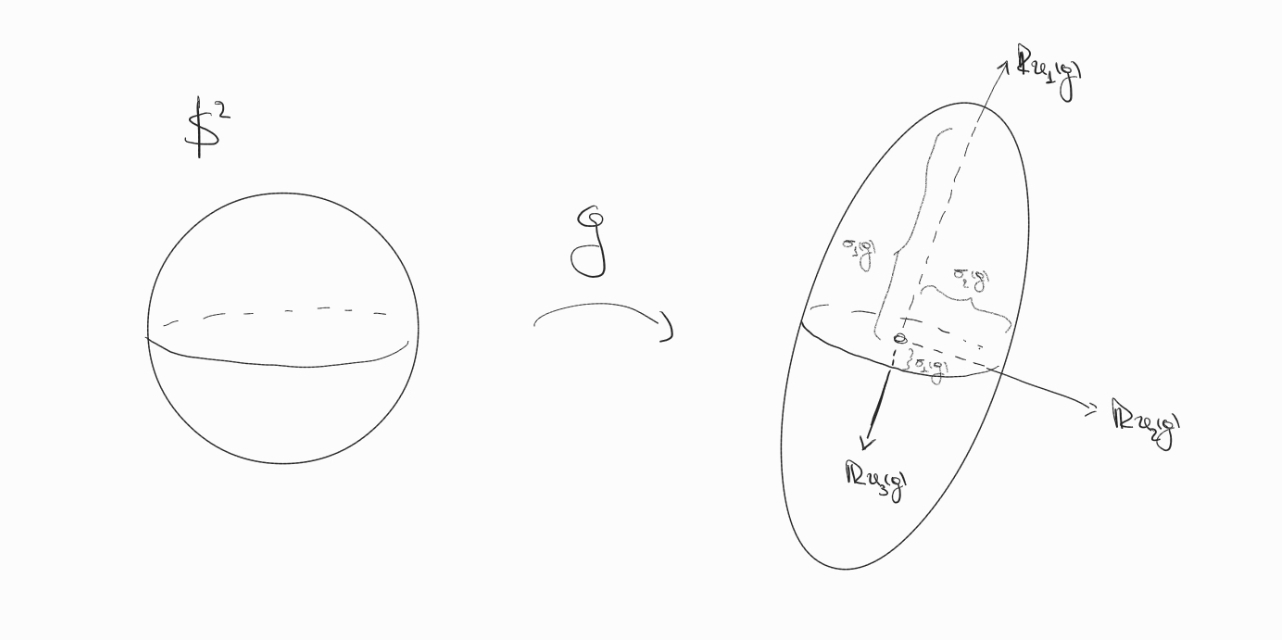
\includegraphics[width=\textwidth]{ball_streching.jpg}
    \caption{Linear transformations map spheres to elllipsoids.}
    \label{fig:ball_stretching}
\end{figure}

In other words, we claim that the image of the unit sphere through $g$ is an ellipsoid with axes
\[
u_i(g) = k_g e_i, \text{ for } i \in \llbracket 1, d \rrbracket
\]
and respective lengths $\sigma_i(g) = e^{\lambda_i(g)}$.
Indeed, if we write $w = \beta_1 u_1(g) + \cdots + \beta_d u_d(g)$, then $w \in g \cdot \mathbb S^{d-1}$ if and only if 
\begin{align*}
    \| g^{-1}w \|^2 &= \| \beta_1 \sigma_i(g)^{-1} l_g^{-1} + \cdots + \beta_d \sigma_d(g)^{-1}\|^2 =\\
    &= \left(\frac{\beta_1}{\sigma_1(g)}\right)^2 + \cdots + \left(\frac{\beta_d}{\sigma_d(g)} \right)^2 \leq 1,
\end{align*}
which is precisely the defining inequality for an ellipsoid.

Recall that for a general element in $g \in \SL(d, \mathbb R)$, we may not make any assumption on the singular values $\sigma_i(g)$ except from the fact that they are in non-increasing order.
In particular, certain singular values may coincide, which in the context of the above discussion means that the choice of the axes $u_i(g)$ is arbitrary.
In fact, when for instance $\sigma_2(g) = \sigma_3(g)$, any rotation of the orthonormal basis on the $\mathbb R u_i(g) \oplus \mathbb R u_{i+1}(g)$ plane will give the equally valid orthonormal choice of axis $u_1(g), \cos(\theta) u_1(g) + \sin(\theta) u_2(g), -\sin(\theta) u_1(g) + \cos(\theta) u_2(g), u_3(g), \cdots, u_d(g)$.
This has to do with the fact that the choice of elements $k_g, l_g$ in the Cartan decomposition of $g$ is not unique (see \cref{fig:arbitrary_axis}).
\begin{figure}[h]
    \centering
    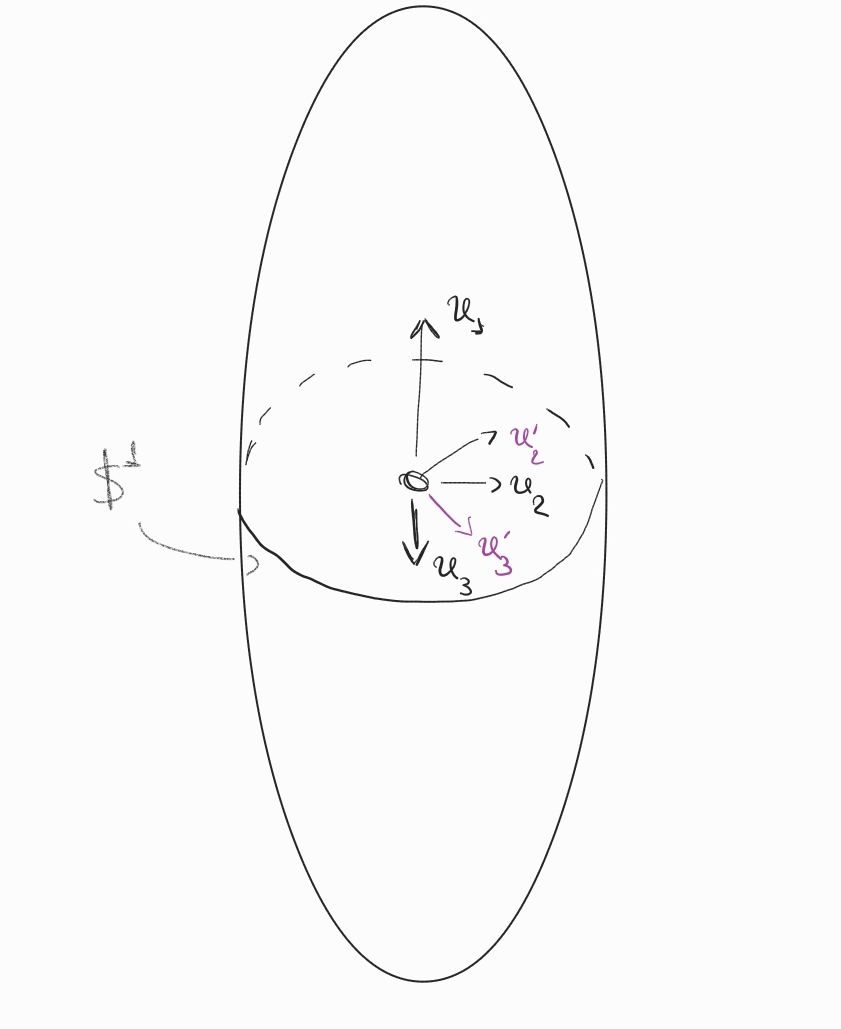
\includegraphics[width=0.4\textwidth]{arbitrary_axis.jpg}
    \caption{Equality between singular values results in axes ambiguity.}
    \label{fig:arbitrary_axis}
\end{figure}

When however there is a singular value gap, i.e.\ $\sigma_p(g) > \sigma_{p+1}(g)$, then (noting that $\sigma_{d-p+1}(g^{-1}) < \sigma_{d-p}(g^{-1})$ as well because $\sigma_i(g^{-1}) = \sigma_{d-i + 1}(g)^{-1}$) the choice of the axis $u_p(g)$ is unique up to a sign, and the attracting and repelling $p$-planes of $g$ are well defined:
\begin{align*}
    U_p(g) &\equaldef k_g \cdot \mathbb R e_1 \oplus \cdots \oplus \mathbb R e_p\\
    U_{d-p}(g^{-1}) &\equaldef l_g^{-1} \cdot \mathbb R e_{p+1} \oplus \cdots \oplus \mathbb R e_d\\
\end{align*}
are well defined and form a decomposition
\[
    g^{-1} \cdot U_p(g) \oplus U_{d-p}(g^{-1})
\]
that is orthogonal with respect to the standard inner product on $\mathbb R^d$.\todo{Prove that attracting flag is well-defined when there exists a singular value gap, and explain that in the bassin, g attracts flags uniformly to the attracting flag} 

In particular, when $g \in \SL(d, \mathbb R)$ has a gap between the $\theta$-th and $(\theta+1)$-th singular values for all $\theta \in \Theta \subseteq \llbracket 1, d-1 \rrbracket$, we define for any $\alpha > 0$ the basin of attraction of $g$ as
\[
B_{\Theta, \alpha}(g) \equaldef \left\{ x \in \mathcal F_{\Theta}(\mathbb R^d) : \angle \left(x^\theta, U_{d-\theta}(g^{-1})\right) \text{ for all } \theta \in \Theta \right\}.
\]
We may think of the basin of attraction as the set of flags that are away from the repelling flag $\left(U_{d-\theta}(g^{-1})\right)_{\theta \in \Theta}$ of $g$.
To justify the name, we briefly mention informally the fact that flags contained in the basin of attraction are uniformly attracted to the attracting flag $U_{\Theta}(g)$ under the action of $g$, and refer to \cite{bochi2019anosov}[Lemma A.6].
Often, for readability purposes, we will often skip writing the curly braces around the indices comprising $\Theta$.

We are now ready to give one of the various equivalent definitions of Anosov representations in the literature.
In light of the previous discussion, one could phrase it as: "a representation in $\SL(d, \mathbb R)$ is $p$-Anosov if the length of the $p$-th axis of the ellipsoid $g \cdot \mathbb S^{d-1}$ is exponentially larger than the length of the $(p+1)$-th axis, with the exponential rate controlled by the word length of the group element". 
\begin{definition}\label{def:anosov}
    Let $\rho: \Gamma \to \SL(d, \mathbb R)$ be a linear representation and $p \in \llbracket 1, d-1 \rrbracket$.
    We say that $\rho$ is $p$-Anosov if there exist constants $\mu, C>0$ such that for all $\gamma \in \Gamma$:
    \[
        \frac{\sigma_{p+1}}{\sigma_p}(\rho(\gamma)) \leq C e^{-\mu |\gamma|}.
    \]
\end{definition}

The following theorem shows the dynamical behaviour of Anosov representations through their action on flag spaces.
In particular, a $p$-Anosov representation $\rho$ will have a well-defined attracting flag $\xi^p_\rho(x)$ in $\mathcal F_{p, d-p}(\mathbb R^d)$ for every $x \in \partial \Gamma$.
\begin{theorem}[\cite{labourie_anosov_2006,kapovich2017anosov}]\label{thm:boundary_map}
    \index{Anosov!boundary maps}
    Let $\rho: \Gamma \to \SL(d, \mathbb R)$ be a $p$-Anosov representation.
    Then there exists an equivariant continuous map $\xi: \partial \Gamma \to \mathcal F_{p, d-p}(\mathbb R^d) $ such that
    \begin{align*}
        \xi^p(x) &= \lim_{n \to \infty} U_p(\rho(\gamma_n))\\
        \xi^{d-p}(x) &= \lim_{n \to \infty} U_{d-p}(\rho(\gamma_n)),
    \end{align*}
    for any $x \in \partial \Gamma$ and any quasi-geodesic $\gamma_n \to x$, and
    it is dynamics-preserving, i.e.
    \[
    \rho(\gamma_n) z \to x
    \]
    for all quasi-geodesics $\gamma_n$ going from $y$ to $x$ and all $z \in \partial \Gamma \backslash \{ y \}$.
    Moreover, it has the following transversality property on the boudnary: for every $x, y \in \partial \Gamma$, the flags $\xi_\rho(x), \xi_\rho(y)$ are transverse unless $x=y$.
\end{theorem}
Again, we would like to stress that if the elements of the Anosov subgroup did not have the singular value gap, then the attracting flags $U_p, U_{d-p}$ would not be well defined.

The next lemma shows that in the case where $\rho: \Gamma \to \SL(d, \mathbb R)$ is projective Anosov and strongly irreducible, continuity and equivariance of  characterise the boundary map $\xi_1: \SL(d, \mathbb R) \to \mathbb P(\mathbb R^d)$.
\begin{lemma}\label{lem:equivariance_uniqueness}
    Let $\rho: \Gamma \to \SL(d, \mathbb R) $ be a strongly irreducible projective Anosov representation, and denote with $\xi_\rho: \partial \Gamma \to \mathbb P(\mathbb R^d)$ its limit map.
    Then $\xi^1_\rho$ is the unique continuous, $\rho(\Gamma)$-equivariant map from $\partial \Gamma$ to $\mathbb P(\mathbb R^d)$.
\end{lemma}
\begin{proof}
    Let $\eta^1: \partial \Gamma \to \mathbb P(\mathbb R^d)$ be a continuous, $\rho(\Gamma)$-equivariant map.
    Since the action of $\Gamma$ on its boundary $\partial \Gamma$ has dense orbits, it suffices to show that it agrees with $\xi^1_\rho$ on at least one boundary point.

    Suppose for the sake of contradiction that $\eta^1$ does not coincide with $ \xi^1$ and let $z \in \partial \Gamma, y \in \partial \Gamma \backslash \{z\}$.
    Then for any $x \in \partial \Gamma \backslash \{y \}$ we may find some quasi-geodesic $\{\gamma_n\}_n$ such that $\gamma_n \to x, \gamma_{-n} \to y$ as $n \to \infty$.
    Then since $z \neq y$ we know that $\gamma_n z \to x$ as $n \to \infty$ and continuity of $\eta^1$ implies that $\eta^1(\gamma_n z) \to \eta^1(x)$.
    But equivariance of $\eta^1$ and the fact that $\xi^1$ is dynamics-preserving (\cref{thm:boundary_map}) implies that $\eta(\gamma_n z) = \rho(\gamma_n) \eta(z) \to \xi^1(x)$,
    unless $\eta^1(z) \in \xi^{d-1}(y)$.
    But if in fact $\eta^1(z) \not \in \xi^{d-1}(y)$, then the limits would agree, i.e.\ $\eta^1(x) = \xi^1(x)$ which is a contradiction.
    Thus we have that $\eta^1(z) \in \xi^{d-1}(y)$ and since $y$ was an arbitrary points of $\partial \Gamma \backslash \{z\}$, we have that
    \[
    \eta^1(z) \in \bigcap_{y \in \partial \Gamma \backslash \{z\}} \xi^{d-1}(y) \subseteq 
    \bigcap_{y \in \partial \Gamma \backslash \Gamma \cdot z} \xi^{d-1}(y).
    \] 
    In particular, the set appearing on the right hand side is a $\rho$-invariant, non-empty proper subset of $\mathbb R^d$, which contradicts the strong irreducibility assumption of $\rho$.
\end{proof}

\section{Important functionals and definitions}
In this section we will introduce certain functionals on the Weyl chamber, whose critical exponents (see \cref{def:functional_critical_exponent}) is going to generalise the critical exponent of the group to the higher rank case.
\begin{definition}\index{Falconer!functional}\index{unstable Jacobian}
For $p \in \llbracket 2, \ldots, d \rrbracket, s\in \mathbb R $
we define the functionals $\Psi_s^p: \mathfrak a^+ \to \mathbb R$, the Falconer functional $F_s: \mathfrak a^+ \to \mathbb R$, and the unstable Jacobian $J_p^u: \mathfrak a^+ \to \mathbb R$ as follows:
\begin{align*}
\Psi_s^p &= 
    {\sf a}_{1,2} + \cdots + {\sf a}_{1,p-1} + (s - (p-2)){\sf a}_{1,p}\\
F_s(a) &= \min 
    \left\{
        \sum_{j=2}^d s_j \alpha_{1,j}(a) : s_j \in (0,1], \sum_{j=2}^d s_j = s 
    \right\}\\
J_p^u &= (p+1)\omega_1 - \omega_{p+1} =
{\sf a}_{1,2} + \cdots + {\sf a}_{1,p+1}.
\end{align*}
\end{definition}

\begin{lemma}\label{lem:functional_relations}
The functionals defined above are related as follows:
\begin{align*}
    F_s(a) &= \max_{p \in \llbracket 2, d \rrbracket} \Psi_s^p(a) = \Psi_s^{p_0}(a) \text{ for } s \in [p_0 - 2, p_0 -1]. \text{ for all } a \in \mathfrak a^+\\
    \frac{s}{p} J_{p}^u &\leq \Psi_{s+p}^{p + 1} \text{ for all } s > 0
\end{align*}
\end{lemma}
\begin{proof}
Indeed, a quick calculation shows that for $s \geq 0, p \in \llbracket 2, d \rrbracket$ and $a \in \mathfrak a^+$ we have that:
\[
    \Psi_s^p(a) \leq \Psi_s^p(a) \text{ if and only if } s \geq p-1.
\]
and that equality holds in the case $s = p - 1$.
Thus for $s \in [p - 2, p-1]$ we have that
\begin{align*}
    s \geq p-2, \ldots, 1 &\text{ implies that } \Psi_s^p(a) \geq \ldots \geq \Psi_s^{2}(a)\\
    s \leq p, \ldots, d-1 &\text{ implies that } \Psi_s^p(a) \leq \ldots \leq \Psi_s^d(a)
\end{align*}
Another way to see this (refer to \cref{fig:max}) is to note that $\Psi_s^2(a), \cdots, \Psi_s^d(a)$ is a sequence of functions that are affine in $s$, with slopes $\alpha_{12}(a) \leq \cdots \leq \alpha_{1d}(a)$ and that they satisfy $\Psi_1^2(a) = \Psi_2^2(a), \Psi_2^3(a) = \Psi_3^4(a) \ldots, \Psi_{d-2}^{d-1}(a) = \Psi_{d-2}^d(a)$.
\begin{figure}[h]
    \centering
    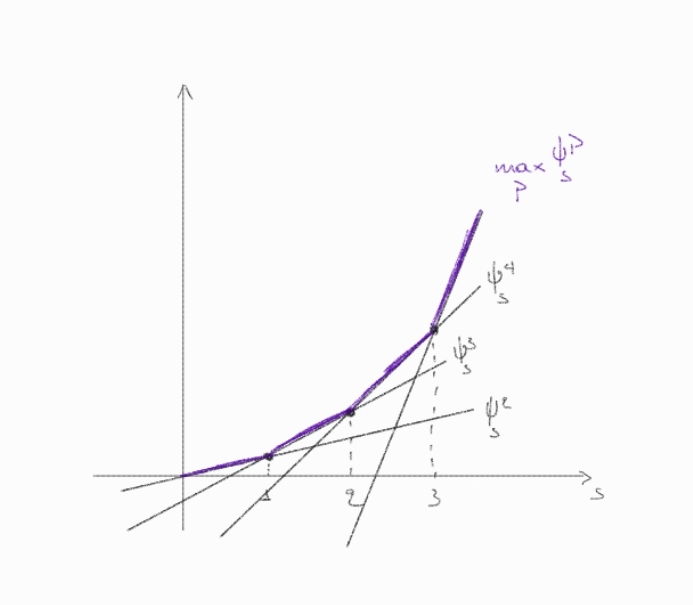
\includegraphics[width=0.4\textwidth]{max.jpg}
    \caption{Visual illustration that $\max_p\Psi_s^p(a) = \Psi_s^{p_0}(a) \text{ for } s \in [p_0 - 2, p_0 -1]$.}
    \label{fig:max}
\end{figure}

For the inequality, the calculations has as follows:
\begin{align*}
    \Psi_s^{p + 1} &=
    {\sf a}_{1,2} + \cdots + {\sf a}_{1,p + 1} + (s-p) {\sf a_{1,p+2}}\\
    &= 
    {\sf a}_{1,2} + \cdots + {\sf a}_{1,p + 1} + p\left(\frac{s}{p}-1\right) {\sf a_{1,p+2}}\\
    &\geq
    {\sf a}_{1,2} + \cdots + {\sf a}_{1,p + 1} + \left(\frac{s}{p}-1\right) ({\sf a}_{1,2} + \cdots + {\sf a}_{1,p + 1})\\
    &=
    \frac{s}{p} J_{p}^u.
\end{align*}

\end{proof}
\begin{remark}
    The reason to consider the functionals $\Psi_s^p, F_s$ will be apparent in \cref{ch:upper_bound}, where we prove that the Hausdorff dimension of the limit set is bounded above by the critical exponent of the Falconer functional.
    There, we will see that the sums in the left-hand-side of the equality
\begin{align*}
    \min_{p \in \llbracket 2, d \rrbracket} 
    \left\{ 
        \sum_{|\gamma| = T} 
            \frac{\sigma_2}{\sigma_1}\cdots\frac{\sigma_{p-1}}{\sigma_1}(g) 
            \left( \frac{\sigma_{p-1}}{\sigma_1}(g) \right)^{s - (p-2)}
    \right\} = 
    \sum_{|\gamma| = T} e^{-F_s(a(g))}
\end{align*}
correspond to the Hausdorff content of respective coverings of $\xi_\rho^1(\partial \Gamma)$ by projective ellipses of different lengths.
For the use of the unstable Jacobian $J_p^u$ we refer to \cref{sec:ProofStrategy}.
\end{remark}

As described in the begining of this section, some of the core objects that we will be working with are critical exponents and Hausdorff dimensions, which we recall below:
\begin{definition}\index{critical exponent!of functional}
    \label{def:functional_critical_exponent}
Let $\phi \in \mathfrak (a^+)^*$ be a functional over the Weyl chamber and $\Gamma \leq \SL(d, \mathbb R)$ a discrete subgroup.
We define the critical exponent of $\phi$ over $\Gamma$ to be
\[
    h_\Gamma(\phi) = \inf
    \left\{
        s > 0: \sum_{\gamma \in \Gamma} e^{-\phi(\gamma)} < \infty
    \right\}.
\]    
\end{definition}

\begin{example}
    \label{ex:critical_exponent}
    \todo{Is this true for Cartan subalgebras of rank-1 Lie groups?}
    Let $\Gamma$ be a uniform lattice of $\SO(1, d)$.
    Then any functional $\phi \in \mathfrak a^*$ is of the form
    \[
        \phi(\mu(\gamma)) = d_\phi(\gamma \cdot o, o) 
    \]
    for some distance $d_\phi$ on $\mathbb H^d$.
    In particular, fixing some $\phi \in \mathfrak a^*$ such that $d_\phi = d$, we have that
    \[
    h_\Gamma(\phi) = \delta_\Gamma.
    \] 
\end{example}

When $\phi = F$ is the Falconer functional, we obtain the following special case (of projective Anosov representations, i.e.\ $P = {1}$) of a definition from \cite{ledrappier_dimension_2023}:
\begin{definition}\index{Falconer!dimension}
    We define the Falconer dimension $\dim_F(\rho)$ of $\rho$ to be the critical exponent of the Falconer functional:
    \[
        \dim_F(\rho) = \inf
        \left\{
            s > 0: \sum_{\gamma \in \Gamma} e^{-F_s(\rho(\gamma))} < \infty
        \right\}.
    \]
\end{definition}

Lastly, we recall the definition of the Hausdorff dimension:
\begin{definition}\index{Hausdorff!dimension}\label{def:hausdorff_dimension}
    Let $(X,\d)$ be a metric space and $A \subseteq X$ be a subset.
    We define the Hausdorff dimension of $A$ to be
    \[
        \dim_{\mathcal H}(A) = \inf
        \left\{
            s > 0: \mathcal H^s_\infty(A) = 0
        \right\},
    \]
    where $\mathcal H^s_\infty$ is the $s$-dimensional Hausdorff content of $A$, defined as
    \[
        \mathcal H^s_\infty(A) = \lim_{\delta \to 0} \inf
        \left\{
            \sum_{i=1}^\infty \diam(U_i)^s: A \subseteq \bigcup_{i=1}^\infty U_i
        \right\}.
    \]
\end{definition}

\section{Hausdorff measures and densities}\label{sec:measures_and_densities}
Let $M$ be a submanifold of a Riemannian manifold $N$.
Depending on the context, there are different ways to define a ``natural'' measure on $M$ in a way that reflects the geometry of $N$, the most common of which are volume forms, densities and the Hausdorff measure.

For instance, when $N$ is an orientable Riemannian manifold, there is a canonical volume form on $N$ which induces a measure on $N$ that can be restricted to $M$.
When however neither $M$ nor $N$ is orientable, there exists no volume form that we can integrate.
In this case, one can use a Riemannian density on $N$, which is a generalisation of differential forms, to obtain a measure on $N$ and then restrict it to $M$.
Alternatively, one could use the restriction on $M$ of the Riemann metric on $N$ to define the Hausdorff measure on $M$.
The reason that we are interested in these methods is that they allow us to define a measure not only in the case where $M$ and $N$ are non-orientable, but also in the case where $M$ is a Lipschitz submanifold, meaning that its tangent spaces are well-defined almost everywhere.

We begin by recalling the necessary material from the theory of densities, which can be found for instance in \cite{lee2012smooth}. 
Seeing the following definition, it is apparent that densities are a generalisation of differential forms, in the sense that they are functions that obey the transformation law of differential forms.
Note however that this is a strict generalisation, as densities need not to be linear in any of their coordinates. 
\begin{definition}
    Let $V$ be a vector space.
    A density on $V$ is a function
    \[
    \mu: V\times \cdots \times V \to \mathbb R
    \]
    such that for every linear transformation $T: V \to V$ and every $v_1, \ldots, v_n \in V$ we have
    \[ 
    \mu(Tv_1, \ldots, Tv_n) = |\det T| \mu(v_1, \ldots, v_n).
    \]
    We say that it is a positive density on $M$ if it is everywhere non-negative and we denote the set of densities by $\mathcal D(V)$.
\end{definition}
To pass from vector spaces to manifolds, we use the notion of a density bundle, which is a direct analog of the tangent bundle.
For a proof that the density bundle is indeed a line bundle, see \cite{lee2012smooth}[Proposition 16.36].
\begin{definition}
    Let $M$ be a smooth manifold.
    We denisty bundle is the line vector bundle $$\mathcal D(M) \overset{\pi}{\to} M$$ whose fiber at $x \in M$ is the space of densities $\mathcal D(M)_x \equaldef \mathcal D(T_x M)$ on the tangent space $T_x M$, and where $\pi$ is the projection map $\pi_{|T_x M} = x$.
\end{definition}
With the above definition at hand, we will henceforth call a density on $M$ a continous section of the density bundle $\mathcal D(M)$, which 
just like every space of bundle sections, is a $C(M)$-module.
\begin{example}
    Let $M$ be an orientable Riemannian manifold and denote with $\mathrm{Vol}$ is Riemannian volume form.
    Then $M$ admits a natural positive density $|\mathrm{Vol}|$ defined by
    \[
    |\mathrm{Vol}|(v_1, \ldots, v_n) = |\mathrm{Vol}(v_1, \ldots, v_n)|.
    \]
    We call $|\mathrm{Vol}|$ the Riemannian density on $M$.
\end{example}

Just as in the case of differential forms, one can pull-back densities through smooth maps and obtain new ones.
\begin{definition}
    Let $f: M \to N$ be a smooth map between smooth manifolds, and $\mu$ be a density on $N$.
    The pull-back of $\mu$ by $f$ is the density $f^*\mu$ on $M$ defined by
    \[
    (f^*\mu)_x(v_1, \ldots, v_n) = \mu_{f(x)}(df_x v_1, \ldots, df_x v_n),
    \]
    for $v_1, \cdots, v_n \in T_x M$.
\end{definition}

We the above definitions at hand, we may now set out to define the integral of a density $\mu$ over a manifold $M$.
We begin by considering the case of a density $\mu$ on $M = \mathbb R^d$, whose support is contained in the closure $\overline{U}$ of an open set $U \subseteq \mathbb R^d$.
Then there exists a unique continuous function $f: \mathbb R^d \to \mathbb R$ such that $\mu = f |\d x_1 \wedge \cdots \wedge \d x_d|$ and we define
\[
\int_D \mu = \int_D f \d x_1 \cdots \d x_d.
\]
To extend this definition to any smooth manifold $M$, we need to show that it is invariant under diffeomorphism:
\begin{proposition}
    Suppose $U, V$ are open subsets of $\mathbb R^n, f: U \to V$ is a diffeomorphism and $\mu$ is a compactly supported density on $V$.
    Then
    \[
    \int_U f^*\mu = \int_V \mu.
    \]
\end{proposition}
Letting now $M$ be a smooth $n$-manifold, for a density $\mu$ that is compactly supported in a coordinate chart $(U, \phi)$ of $M$, we define:
\[
\int_M \mu = \int_{\phi(U)} (\phi^{-1})^*\mu.
\]
and extend this to any density $\mu$ on $M$ by
\[
\int_M \mu = \sum_{i} \int_M \psi_i \mu,
\]
where $\{\psi_i\}$ is a partition of unity subordinate to a cover of $M$ by coordinate charts.

We now apply the theory of densities to the case of a space of partial flags.
Before we do so, recall that the tangent space to 
\begin{example}
    Let $p \in \llbracket 2, d-1 \rrbracket, V \in V \in \mathcal G_{p}{\mathbb R^d}$ and $l \in \mathbb P(V)$.
        Using the canonical identification $T_l \mathbb P(V) \simeq \hom (l, V/l)$, we define the density $|\Omega|$ over $\mathcal F_{1, p}(\mathbb R^d)$ by
    \[
        |\Omega_{l,V}|(\phi_1, \ldots, \phi_p) = 
        \frac{\| v \wedge \tilde \phi_1(v) \wedge \cdots \wedge \tilde \phi_p (v) \|}{\|v\|^{p+1}}
    \]
    for any $v \in l - \{ 0\}$, where $\tilde \phi_1, \ldots \tilde \phi_p \in \hom(l, V)$ are such that $\phi_i = \tilde \phi_i + \hom(l, l)$ and $\| \cdot \|$ denotes the norm on $\bigwedge^{p+1} \mathbb R^d$ induced by the standard euclidean inner product.
\end{example}

\todo{Add some theory on densities and show that the density on $\mathcal F_{1. p+1} (mathbb R^d)$ is $\SL(d, R)$ equivariant}

\section{Complex hyperbolic geometry}\label{sec:complex_geometry}
In this section we gather some material on complex hyperbolic geometry that will be useful in providing a counterexample to a lemma of \cite{pozzetti_anosov_2023} in \cref{sec:two_counterexamples}.
Although we will focus on the complex hyperbolic plane, in most cases, the same facts will also hold for higher dimensional complex hyperbolic spaces.
For proofs of what we are about to recall, the reader can refer to any introductory source on the matter, such as \cite{parker2003notes}.

The complex hyperbolic plane\index{complex hyperbolic plane} $\mathbb H^2_{\mathbb C}$ admits several equivalent models, according to the Hermitian form\index{Hermitian form} that is used to define it.
For completenes, we recall that a Hermitian form over a complex vector space $V$ is a mapping $V\times V \to \mathbb C$ that is linear in the first term and conjugate linear in the second.
Each such form $\langle \cdot, \cdot \rangle$ is associated to a Hermitian matrix $A$ (meaning that $A^* = A$) in the sense that $x^* A y = \langle x, y \rangle$ for all $x, y \in V$.
The following example lists the Hermitian forms that we will be using:
\begin{example}
    For $z, w \in \mathbb C^3$ we have the following two forms of signature $(2,1)$:
    \begin{align*}
        \langle z, w \rangle_1 &= z_1 \overline{w_1} + z_2 \overline{w_2} - z_3 \overline{w_3}\\
        \langle z, w \rangle_2 &= z_1 \overline{w_3} + z_2 \overline{w_2} + z_3 \overline{w_1}
    \end{align*}
    which correspond to the matrices
    \[
    J_1 = \begin{pmatrix}
        1 & 0 & 0\\
        0 & 1 & 0\\
        0 & 0 & -1
    \end{pmatrix} \quad \text{ and } \quad
    J_2 = \begin{pmatrix}
        0 & 0 & 1\\
        0 & 1 & 0\\
        1 & 0 & 0
    \end{pmatrix}.
    \]
\end{example}

We will denoting with $\mathbb C^{2,1}$ the space $C^3$ equipped with a $(2,1)$-Hermitian form $\langle \cdot, \cdot \rangle$ and with $\SU(2,1) \leq \SL(2, \mathbb C)$ its isometries.
Then the projective model for the hyperbolic plane $\mathbb H^2_{\mathbb C}$ is the set of all negative lines in $\mathbb C^{2,1}$ and its boundary $\partial \mathbb H^2_{\mathbb C}$ is the set of all isotropic lines:

\begin{align*}
    \mathbb H^2_{\mathbb C} &\equaldef \left\{ [z_1: z_2: z_3] \in \mathbb P(\mathbb C^{2,1}): \langle z, z \rangle < 0 \right\},\\
    \partial \mathbb H^2_{\mathbb C} &= \left\{ [z_1: z_2: z_3] \in \mathbb P(\mathbb C^{2,1}): \langle z, z \rangle = 0 \right\}.
\end{align*}

Let us for the moment consider the projective model as defined from the Hermitian form $\langle \cdot, \cdot \rangle_2$.
In that case, the metric on $\mathbb H^2_{\mathbb C}$ is called the Bergman metric\index{Bergman metric} and is given by the relation
\[
\cosh(\frac{d(z,w)}{2}) = \frac{\langle z, w \rangle \langle w, z \rangle}{\langle z, z \rangle \langle w, w \rangle}.
\]\todo{Why is this the Bergman metric?}
The set of isometries\index{$\SU(2,1)$} is given by the rank 1 Lie group
\[
\SU(2,1) \equaldef \left\{ g \in \SL(3, \mathbb C) : g^* J_2 g = J_2 \right\},
\]
with Lie algebra
\begin{align*}
    \su(2,1) &= \left\{ g \in \gl(3, \mathbb C) : g^* J_2 = - J_2 g, \tr(g) = 0 \right\}\\
    &= \left\{ 
        \begin{pmatrix}
            u - is & a & it\\
            b & 2is & -\overline{a}\\
            ir & -\overline{b} & -u - is
        \end{pmatrix} : u,r,s,t \in \mathbb R, a, b \in \mathbb C
    \right\}.
\end{align*}
The maximal compact subgroup that we will work with will be the stabiliser of $[1:0:-1]$ in $\SU(2,1)$ and will be denoted with $K$.

From the above expression of $\su(2,1)$, we obtain an ordered basis of $\su(2,1)$
\[
    \su(2,1) = \spa\left\{\begin{array}{lllll}
        &\begin{pmatrix}
            1 & 0 & 0\\
            0 & 0 & 0\\
            0 & 0 & -1
        \end{pmatrix},
        &i\begin{pmatrix}
            -1 & 0 & 0\\
            0 & 2 & 0\\
            0 & 0 & -1
        \end{pmatrix},
        &\begin{pmatrix}
            0 & 1 & 0\\
            0 & 0 & -1\\
            0 & 0 & 0
        \end{pmatrix},
        &i\begin{pmatrix}
            0 & 1 & 0\\
            0 & 0 & 1\\
            0 & 0 & 0
        \end{pmatrix},\\~\\
        &i\begin{pmatrix}
            0 & 0 & 1\\
            0 & 0 & 0\\
            0 & 0 & 0
        \end{pmatrix},
        &\begin{pmatrix}
            0 & 0 & 0\\
            1 & 0 & 0\\
            0 & -1 & 0
        \end{pmatrix},
        &i\begin{pmatrix}
            0 & 0 & 0\\
            1 & 0 & 0\\
            0 & 1 & 0
        \end{pmatrix},
        &i\begin{pmatrix}
            0 & 0 & 0\\
            0 & 0 & 0\\
            1 & 0 & 0
        \end{pmatrix}
    \end{array}\right\}.
\]
in which a tedious calculation yields
\[
\ad \begin{pmatrix}
    1 & 0 & 0\\
    0 & 0 & 0\\
    0 & 0 & -1
\end{pmatrix} = \diag(0, 0, 1, 1, 2, -1, -1, -2) \in \gl{\su(2,1)}.
\]

The Cartan subalgebra and Weyl chamber are given by
\[
    \mathfrak a^+ = \mathbb R \cdot \begin{pmatrix}
        1 & 0 & 0\\
        0 & 0 & 0\\
        0 & 0 & -1
    \end{pmatrix} \text{ and }
\mathfrak a^+ = \mathbb R_{\geq 0} \cdot \begin{pmatrix}
    1 & 0 & 0\\
    0 & 0 & 0\\
    0 & 0 & -1
\end{pmatrix} \text{ respectively}.
\]\todo{How do we show that this is the Cartan subalgebra?}

It will be useful later to have an explicit expression of the Cartan projection
\begin{lemma}\label{lem:cartan_projection_su_2_1}
    The Cartan projection $\mu: \su(2,1) \to \mathfrak a^+$ is given by
    \[
    \mu\left(g\right) = \frac{d(g [1:0:-1], [1:0:-1])}{2} \begin{pmatrix}
        1 & 0 & 0\\
        0 & 0 & 0\\
        0 & 0 & -1
    \end{pmatrix}.
    \]
\end{lemma}
\begin{proof}
    Let $g \in \SU(2,1)$.
    Since $\rk(\SU(2,1)) = 1$, there exist $r(g) \in \mathbb R$ and $k, l \in K$ such that
    \[
    g = k e^{\mu(g)} l \text{ and } \mu(g) = r(g) \begin{pmatrix}
        1 & 0 & 0\\
        0 & 0 & 0\\
        0 & 0 & -1
    \end{pmatrix}.
    \]
    To calculate $r(g)$, we note that 
    \begin{align*}
        d\left(g[1:0:-1], [1:0:-1]\right) &= d\left(e^{\mu(g)}[1:0:-1], [1:0:-1]\right) \\
        &= d\left([e^{r(g)}:0:-e^{-r(g)}], [1:0:-1]\right),
    \end{align*}
    and compute it through the relation defining the Bergman metric:
    \[
    \cosh^2\left( \frac{d^2\left([e^{r(g)}:0:-e^{-r(g)}], [1:0:-1]\right)}{2} \right) = \frac{4 \cosh^2{r(g)}}{2 \cdot 2},
    \]
    from which we infer that $d\left([e^{r(g)}:0:-e^{-r(g)}], [1:0:-1]\right) = 2 r(g)$.
\end{proof}

In particular, we claim that since $\Gamma$ is a uniform lattice os $\SU(2,1)$, we have that $\partial \Gamma$ is homeomorphic to $\SU(2,1)/P$, where $P$ is a parabolic subgroup of $\SU(2,1)$, and it coincides with the stabilizer of some isotropic line $l \in \partial_\infty \mathbb H^2_\mathbb C$.

Moving on to parabolic subgroups, we first show how they can be used to obtain the boundary of the complex hyperbolic plane.
\begin{lemma}\label{lem:lattice_boundary}
    Let $\Gamma$ be a uniform lattice of a Lie group $\SU(2,1)$ and $P$ be a parabolic subgroup of $\SU(2,1)$.
    Then the Gromov boundary of $\Gamma$ is homeomorphic to the quotient $\SU(2,1)/P$.  
\end{lemma}
\begin{proof}
    The Milnor-Švarc lemma implies that for any $x_0 \in X$, the map $\Gamma \to X, \gamma \mapsto \gamma x_0$ is a quasi-isometry.
    Since both spaces are Gromov hyperbolic, the quasi-isometry extends to a homeomorphism $\partial \Gamma \to \partial H^2_{\mathbb C}$ of the Gromov boundaries.
    On the other hand, the action of $\SU(2,1)$ on $\partial H^2_\mathbb C$ is transitive and $P$, being a parabolic subgroup, equals the stabiliser of some isotropic line $l \in \partial \mathbb H^2_{\mathbb C}$, so we have that $\partial H^2_{\mathbb C} \simeq \SU(2,1)/P$.
\end{proof}
In latere chapters, we will work with the parabolic subgroup given by $P = \Stab_{\SU(2,1)}([1:0:0])$,whose algebra is
\[
\mathfrak p = \Stab_{\su(2,1)}([1:0:0]) = \left\{
    \begin{pmatrix}
        u - is & a & it\\
        0 & 2is & -\overline{a}\\
        0 & 0 & -u - is
    \end{pmatrix} : u,s,t \in \mathbb R, a \in \mathbb C
\right\}.
\]
\chapter{Upper bound}\label{ch:upper_bound}
In this section we prove the upper bound on the Hausdorff dimension, namely that for a projective Anosov representation in $\SL(d, \mathbb R)$, the Hausdorff dimension of the limit set is bounded above by the Falconer dimension:
\begin{replemma}{lem:upper_bound}[Upper bound for dimension]
    Let $\rho: \Gamma \to \SL(d, \mathbb R)$ be a projective Anosov representation. 
    Then:
    \[
        \dim_{\mathcal H}(\xi^1 (\partial \Gamma) ) \leq h_{\rho(\Gamma)}(F).
    \]
\end{replemma}
    
The idea of the proof is to find a covering whose Hausdorff content is dominated by the Dirichlet series of some functional $\Psi_s^p$, which will in turn imply that $\dim_{\mathcal H}(\xi^1(\partial \Gamma)) \leq h_{\rho(\Gamma)}(\Psi^p) $.
Choosing then the most ``effective'' cover (i.e.\ the one which yields the smallest Hausdorff content up to a constant) we obtain that
\[
    \dim_{\mathcal H}(\xi^1(\partial \Gamma)) \leq h_{\rho(\Gamma)}(F) = h_{\rho(\Gamma)} \left(\max_p \Psi^p \right)
\]
To obtain this we first cover $\xi^1(\partial \Gamma)$ by the shifted bassins of attraction $\rho(\gamma) \cdot B_{\alpha_1, \alpha} (\rho(\gamma))$ for $\gamma \in \Gamma$ satisfying $|\gamma| = T$.
Then, for each $p \in \llbracket 2, d \rrbracket$, the set $\rho(\gamma) \cdot B_{\alpha_1, \alpha} (\rho(\gamma))$ is contained in an ellipsoid of axes lengths
\[
    \beta_2 = \frac{1}{\sin(\alpha)} \frac{\sigma_2}{\sigma_1}(\rho(\gamma)), \ldots, 
    \beta_d = \frac{1}{\sin(\alpha)} \frac{\sigma_d}{\sigma_1}(\rho(\gamma)).
\]
which in turn is covered by roughly $\beta_2 \cdots \beta_{p-1}/\beta_p^{p-2}$ balls of radius $\sqrt{d-1} \beta_p$.
Using this cover to bound the Hausdorff content of $\xi_\rho^1(\partial \Gamma)$, we obtain the bound
\[
    \mathcal H^s(\xi^1(\partial \Gamma)) \lesssim \sum_{|\gamma| = T} e^{-\Psi_s^p(\rho(\gamma))} \leq \sum_{|\gamma| = T} e^{-F_s(\rho(\gamma))}.
\]
If we assume that $s > h_{\rho(\Gamma)}(F)$, then the right-hand side of the inequality converges to zero as we let $T \to \infty$, which means that $\mathcal H^s(\xi_\rho^1(\partial \Gamma)) = 0$, giving us the desired bound.
Finally for each $q \in \llbracket 2, d \rrbracket$, we cover each ellipsoid by balls of some of radius $\beta_q$.


\section{Lemmata}
To simplify the proof of the bound, we present a few preliminary facts in the form of lemmata, whose proofs constitute the matter of this section.
Our first goal will be to obtain an open cover for the limit set using basins of attraction of elements in the Anosov subgroup at a fixed distance from the identity.
It appears as \cite[Proposition 3.5]{pozzetti_anosov_2023}.
\begin{lemma}\label{lem:boundary_covering}
Let $\rho: \Gamma \to SL(d, \mathbb R)$ be projective Anosov.
Then for $\alpha > 0$ small enough, there exists some $T_0 > 0$ such that for all $T \geq T_0$ the family
\[
    \mathcal U_T = \left\{ \rho(\gamma) B_{\alpha_1, \alpha}(\rho(\gamma)) : |\gamma| = T \right\}
\]
is an open covering of $\xi^1(\partial \Gamma)$.
\end{lemma}
To prove this, we will need the following lemma (\cite[Lemma 2.4]{pozzetti_anosov_2023}).
It essentially tells us that if we evaluate an Anosov representation at two points of a geodesic passing from $e \in \Gamma$ that are far apart, then the attracting line at one point is uniformely (with respect to geodesics) far apart from the attracting hyperplane at the other point.
\begin{lemma}\label{lem:angle}
    Let $\rho: \Gamma \to \SL(d, \mathbb R)$ be a projective Anosov representation.
    For $\alpha > 0$ small enough, there exists $T>0$ such that for any geodesic ray $(a_j)_{j \in \mathbb N}$ through $e$ we have:
    \[
        \angle(U_1(\rho(a_i)), U_{d-1}(\rho(a_0))) > \alpha
    \]
    when $|a_i|, |a_0| > T$.
\end{lemma}
\begin{proof}
Assume the contrary for the sake of contradiction.
Then (see Figure \ref{fig:angle} ) for each $n>0$, there exists a geodesic ray  $(a^n)_{j \in \mathbb N}$ through $e$ such that 
\[
    |a_n^n|, |a_0^n| > n \text{ and }
    \angle(U_1(\rho(a_n^n)), U_{d-1}(\rho(a_0^n))) < \frac{1}{n}.
\]
Due to compactness of $\Gamma \cup \partial \Gamma$ we can find some subsequence  ${k_n}$ and $x,y \in \partial \Gamma$ such that $a^{k_n}_{k_n} \to x$, $a^{k_n}_0 \to y$.
Since there exists a geodesic joining $a_{k_n}^{k_n}, a_0^{k_n}$ passing from $e$, we also know that $x\neq y$.
Also, the limit map being continuous (\cref{thm:boundary_map}), we have that
\[
    \angle (\xi^1(x), \xi^{d-1}(y)) = 0,
\]
which contradicts its transversality property.
\end{proof}
\begin{figure}[h]
    \centering
    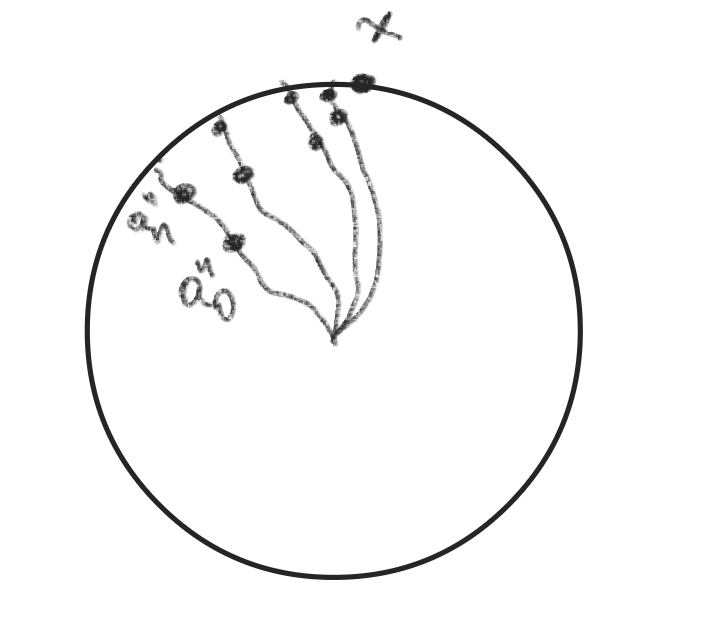
\includegraphics[width=0.3\textwidth]{angle.jpg}
    \caption{Situation in \cref{lem:angle}}
    \label{fig:angle}
\end{figure}    
We may now proceed with the proof of \cref{lem:boundary_covering}:
\begin{proof}[Proof of \cref{lem:boundary_covering}]
    Let $\alpha, T > 0$ be as in the statement of \cref{lem:angle} and $x \in \partial \Gamma$ be represented by a geodesic ray $(\gamma_j)_{j\geq 0}$ starting from $e$.
    Then $(\gamma_T^{-1} \gamma_j)_j$ is a geodesic ray starting from $(\gamma_T)^{-1}$ that passes through $e$, so
    \[
        \angle (U_1(\rho(\gamma_T^{-1}\gamma_j)), U_{d-1}(\rho(\gamma_T^{-1}))) > \alpha
    \]
    as implied by \cref{lem:angle}.
    Taking the limit $j \to \infty$ and using the equivariance of the limit map, we obtain
    \[
        \angle (\rho(\gamma_T^{-1})\xi^1(x), U_{d-1}(\rho(\gamma_T^{-1}))) > \alpha
    \]
    and thus $\xi^1(x) \in \rho(\gamma_T) \cdot B_{\alpha_1, \alpha}(\rho(\gamma_T))$.
\end{proof}

The next step will be to cover each of the sets in $\mathcal U_T$ by ellipsoids in the projective space, which are merely the projectivisation of the usual ellipsoids in $\mathbb R^d$.
Note that while in the case of the latter, the axes are lines (for instance $\mathbb Re_1, \ldots, \mathbb Re_d$), their projective analogue should be planes (for instance $\mathbb R u_1 \oplus \mathbb R u_2, \ldots \mathbb R u_1 \oplus \mathbb R u_d$).
\todo{Does this clarifying comment on the axes of the ellipsoid help?}
\begin{definition}\index{ellipsoid}
    Let $V$ be a finite-dimensional $\mathbb R$-vector space.
    We consider a decomposition
    \[
        V = \mathbb R u_1 \bigoplus \cdots \bigoplus \mathbb R u_d
    \] 
    that is orthogonal with respect to a fixed inner-product over $V$.
    Given $\beta_2 \geq \ldots \beta_d > 0$, we define an ellipsoid with axes $\left(u_1 \oplus u_p\right)_{p \in \llbracket 2, d \rrbracket}$ and lengths $(\beta_p)_{p \in \llbracket 2, d \rrbracket}$ to be the image of
    \[
        \left\{
            v = \sum_1^d v_i u_i\in V : \sum_2^d \left( \frac{v_j}{\beta_j} \right)^2 \leq 1
        \right\}
    \]
    through the projection $ V \to \mathbb P (V)$.
\end{definition}
\begin{figure}[h]
    \centering
    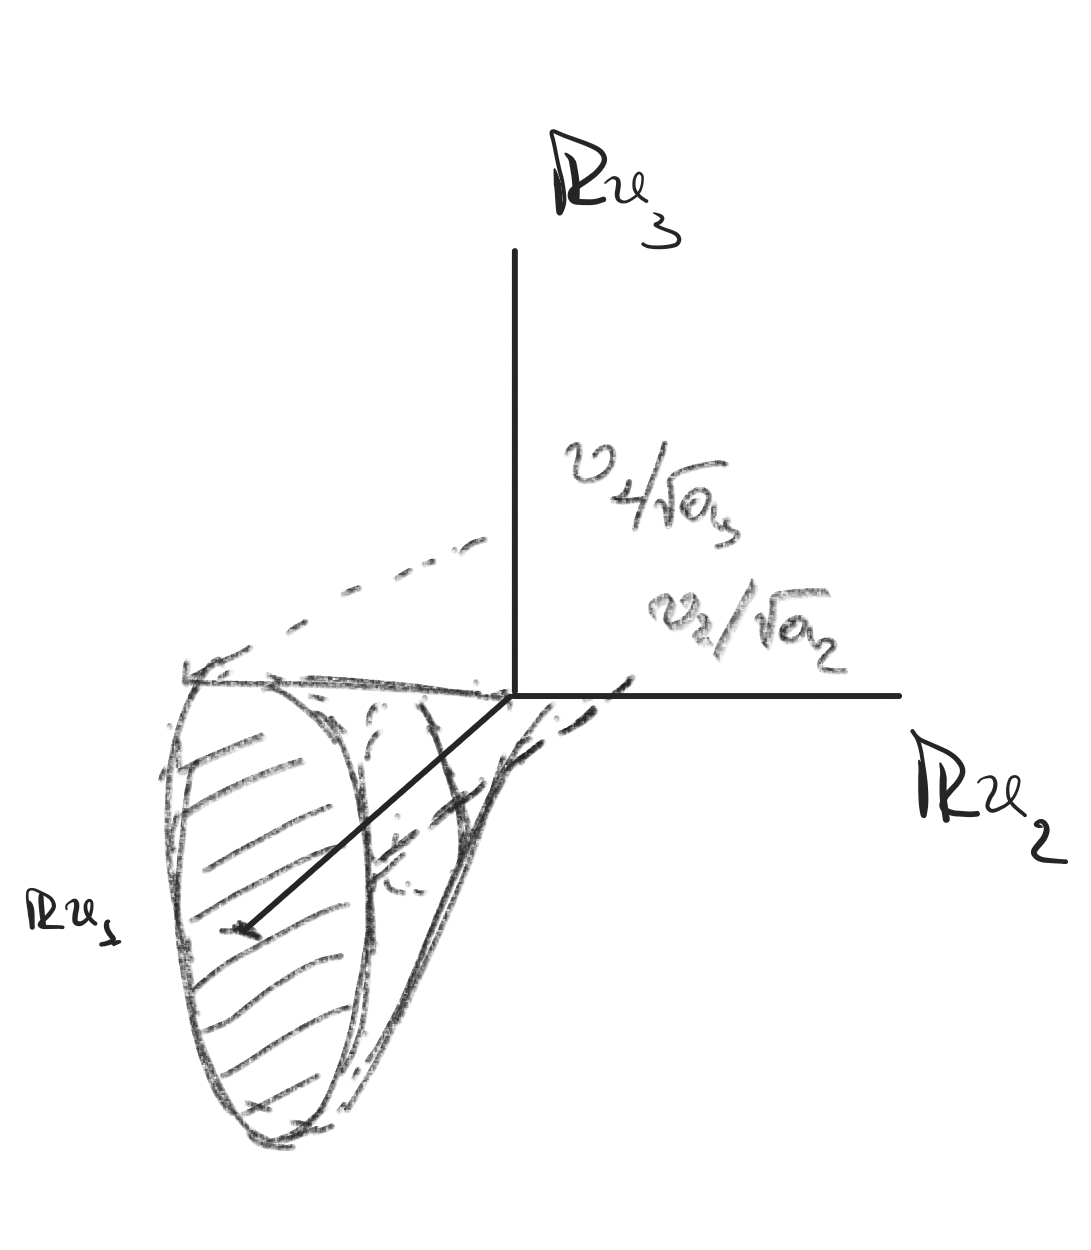
\includegraphics[width=0.4\textwidth]{ellipsoid.jpg}
    \caption{Depiction in $\mathbb R^3$ of an ellipsoid of $\mathbb P(\mathbb R^2)$}
    \label{fig:ellipsoid}
\end{figure}
\todo{Correct ellipsoid drawing}
When we want to distinguish between the projective ellipsoid of the above definition and the usual ellipsoid in $\mathbb R^d$, we will refer to the latter as a euclidean ellipsoid.
When there is no ambiguity, we will simply refer to the projective ellipsoid as an ellipsoid.

The following is \cite[Proposition 3.8]{pozzetti_anosov_2023} and tells us that each set of the covering $\mathcal U_T$ from \cref{lem:boundary_covering} is contained in a projective ellipsoid, whose axes correspond to the axes of the euclidean ellipsoid $g \cdot \mathbb S^{d-1}$, and whose axes depend on the singular values of $g$.
Recalling the discussion preceeding \cref{def:anosov}, it should not come as a surprise since the bassin of attraction is a set of flags that are streched and contracted at a uniform degree under the action of $g$.
\begin{proposition}\label{prop:basin_covering}
Let $g \in \SL(d, \mathbb R), \alpha > 0$, fix a Cartan decomposition $g = k_g e^{\mu(g)} l_g$ and consider the corresponding choice of axes $u_i(g) = k_g e_i, u_i(g^{-1}) = l_g^{-1} e_{d-i+1}$ for $i \in \llbracket 1, d \rrbracket$, along with the respective flags $U_i(g), U_i(g^{-1})$.
Denoting with
\[
B_{{\sf a_1}, \alpha}(g) = \left\{ x \in \mathbb P(\mathbb R^d) : \angle(x, U_{d-1}(g^{-1})) > \alpha \right\}
\]
the bassin of attraction of $g$, the set $g \cdot B_{{\sf a_1}, \alpha}(g)$ lies in the ellipsoid with axes $\left(u_1(g) \oplus u_p(g)\right)_{p \in \llbracket 2, d \rrbracket}$ of lengths
\[
    \frac{1}{\sin \alpha} \cdot \frac{\sigma_p(g)}{\sigma_1(g)}
\]
\end{proposition}
\begin{proof}
Using the definition of the basin of attraction (see \cref{fig:projection} ), for $w \in \mathbb R^d$, we have (up to considering $-w$ instead of $w$) that: 
\[
\angle(\mathbb R w, U_{d-1}(g^{-1})) = \angle(w, w') = \frac{|w_d|}{|w|},
\]
when
\begin{align*}
    w &= w_1 u_1(g^{-1}) + \cdots + w_d u_d(g^{-1})\\
    &= w_1 l_g^{-1} e_c(g) + \cdots + w_d l_g^{-1} e_1(g)\\
\end{align*}
and
\begin{align*}
    w' &= w - w_d u_d(g^{-1}) =\\
    &= w_1 u_1(g^{-1}) + \cdots + w_{d-1} u_{d-1}(g^{-1})\\
    &= w_d l_g^{-1} e_1(g) + \cdots + w_1 l_g^{-1} e_{d-1}(g).
\end{align*}
Then $\mathbb R w \in B_{\alpha_1, \alpha}(g)$ if and only if
\[
    w_d^2 \geq (\sin \alpha)^2 \sum_1^d w_i^2.
\]
Considering now some $v = v_1 u_1(g) + \cdots + v_d u_d(g)$ such that 
$\mathbb R v \in g \cdot B_{\alpha_1, \alpha}(g)$
we have that
\begin{align*}
    w = g^{-1} v &= v_1 \sigma_1(g)^{-1} l_g^{-1} e_1(g) + \cdots v_d \sigma_d(g)^{-1} l_g^{-1} e_d(g)\\
    &= v_1 \sigma_1(g)^{-1} u_{d}(g^{-1}) + \cdots v_d \sigma_d(g)^{-1} u_1(g^{-1})
\end{align*}
where we used that $u_p(g^{-1}) = l_g^{-1} e_{d+1-p}$.
Hence
\[
    \sigma_1(g)^{-2} \cdot v_1^2 \geq (\sin a)^2 \sum_1^d \sigma_i(g)^{-2} v_i^2.
\]
Since the only condition on $v$ is that the line through $v$ lies in $g \cdot B_{\alpha_1, \alpha}(g)$, we may choose $v$ such that $v_1 = \sigma_1(g)$.
Indeed, the only case that this would not be possible is when 
$$v \in \mathbb R(u_2(g) \oplus \cdots u_d(g)) = g U_{d-1}(g^{-1}), $$
which is not possible since this would imply that $g^{-1} v \in U_{d-1}(g^{-1})$.
Thus, the inequality above becomes precisely the condition for $\mathbb R w$ to lie in the projective ellipsoid.
\end{proof}
\begin{figure}[h]
    \centering
    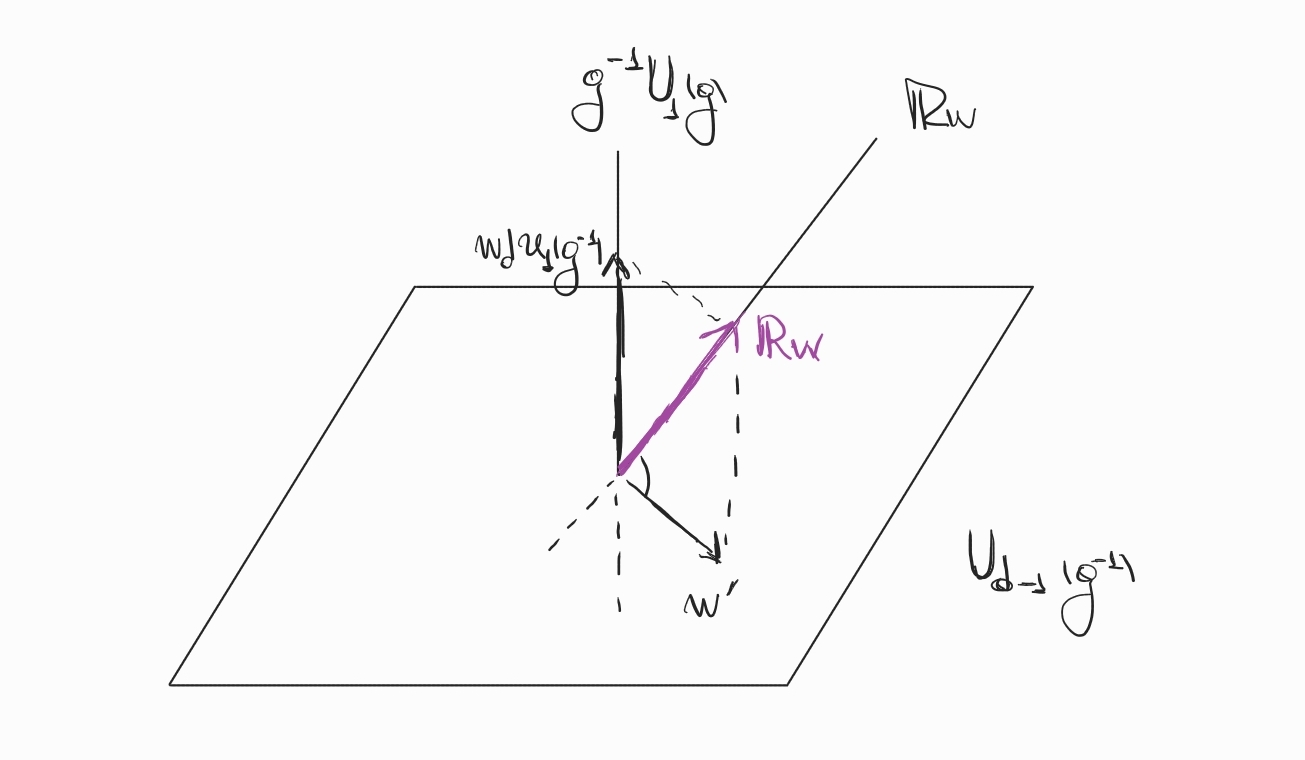
\includegraphics[width=0.6\textwidth]{projection.jpg}
    \caption{Aid for \cref{prop:basin_covering}}
    \label{fig:projection}
\end{figure}

The following is \cite[Lemma 3.7]{pozzetti_anosov_2023}:
\begin{lemma}\label{lem:ellipsoid_covering}
For any $p \in \llbracket 2, d \rrbracket$, an ellipsoid in $\mathbb P(\mathbb R^d)$ of axes lengths $\beta_2 \geq \cdots \geq \beta_d$ is covered by
\[
    2^{p - 2} \frac{\beta_2 \cdots \beta_{p-1}}{\beta_p^{p-2}}
\]
many (projected) balls of radius $\sqrt{d-1} \beta_p$.
\end{lemma}
\begin{proof}
We assume that $E$ is an ellipsoid about $\mathbb R e_1$, so it suffices to cover its intersection $E_1 = E \cap U_1 \subseteq \mathbb R^{d-1}$ with the affine chart $U_1 = \{ [x_1: \ldots, x_d ] \in \mathbb P(\mathbb R^d) : x_1 \neq 0 \}$.
Clearly $E_1 \subseteq [-\beta_2, \beta_2] \times \ldots \times [-\beta_d, \beta_d]$, so we proceed by covering the rectangle with side-lengths $2\beta_2, \ldots, 2\beta_d$.
Clearly each interval $(-\beta_j, \beta_j)$ is contained in the union of $\lceil \beta_j/\beta_p \rceil$ intervals of length $2\beta_p$, thus $E_1$ is contained in the union of
\[
    \left\lceil \frac{\beta_2}{\beta_p} \right\rceil \cdots \left\lceil \frac{\beta_{p-1}}{\beta_p} \right\rceil =
    \left\lceil \frac{\beta_2}{\beta_p} \right\rceil \cdots \left\lceil \frac{\beta_d}{\beta_p} \right\rceil
\]
many squares of side-length $2\beta_p$.
Since each such product is contained in a $(d-1)$-ball of radius $\sqrt{d-1} \beta_p$ we may use at most
\[
    \left\lceil \frac{\beta_2}{\beta_p} \right\rceil \cdots \left\lceil \frac{\beta_{p-1}}{\beta_p} \right\rceil \leq
    \sum_{i \in \{ 0,1 \}^{p-2} } \prod_{j = 2}^{p-1} \left( \frac{\beta_j}{\beta_p} \right)^{i_j} \leq 2^{p-2} \frac{\beta_2}{\beta_p} \cdots \frac{\beta_{p-1}}{\beta_p}
\]
many $(d-1)$-balls of radius $\sqrt{d-1}\beta_p$ to cover $E_1$.
\end{proof}

The following can be found in \cite[Proposition 3.3]{pozzetti_anosov_2023}.
It will not be used until \cref{ch:upper_bound}, but we include it here to stress the fact that (similarly to all results of this chapter and in contrast to the next one) it holds for any projective Anosov representation, without any more assumptions (like Zariski-density of the subgroup or regularity of the limit set).
\begin{proposition}\label{prop:shadows}
    Let $\rho: \Gamma \to SL(d, \mathbb R)$ be projective Anosov and $\alpha > 0$
    Then there exist $c_0, c_1 > 0$ that depends only on $\alpha$ and $\rho$ such that for all $\gamma \in \Gamma$:
    \[
        (\xi^1)^{-1}(B_{\alpha_1, \alpha}(\rho(\gamma))) \subseteq C_{c_0,c_1}^\infty(\gamma)
    \]
\end{proposition}
\begin{proof}
    We begin by noting that it suffices to show this for all but finitely many $\gamma \in \Gamma$, since then we may alter the constants to satisfy the wanted inclusion for the finitely many remaining $\gamma \in \Gamma$ as well. 
    Hence, we may assume that $|\gamma| \geq l_0$ where $l_0 > 0$ is such that 
    \[
        Ce^{-\mu l_0} < 1 \text{ and } {\sf a}_1(\gamma) \geq C|\gamma| - L.
    \]

    Suppose $x \in \partial \Gamma$ such that $\xi^1(x) \in B_{\alpha_1, \alpha}(\rho(\gamma))$, and consider a geodesic ray $a_j \to x$ starting from $a_0 = e$.
    To prove the result, it suffices to find constants $c_0, c_1$ independent of $\gamma$ and for which there exists a ($c_0$, $c_1$)-quasi-geodesic from $\gamma^{-1}$ to $x$ that passes through $e$ and stays at a bounded distance from $(a_j)_{j=0}^\infty$.

    Using the exponential convergence rate of $\xi^1(a_j) \to \xi^1(x)$ and the definition of $B_{\alpha_1, \alpha}(\rho(\gamma))$ we have that:
    \begin{align*}
        d(\xi^1(a_j), \xi^1(\gamma)) &\geq
        d(\xi^1(x), U_1(\rho(\gamma^{-1}))-d(\xi^1(a_j), \xi^1(x)))
        \geq \\
        &\geq
        d(\xi^1(x), U_{d-1}(\rho(\gamma^{-1}))-d(\xi^1(a_j), \xi^1(x)))
        \geq
        \sin \alpha - Ce^{-\mu j}
    \end{align*}
    which along with the uniform continuity of $\xi^1: \Gamma \cup \partial \Gamma \to \mathbb P(\mathbb R^d)$ implies that there exists some $\alpha' > 0$ and $L>0$ such that for all $j\geq L$:
    \[
        d(a_j, \gamma^{-1}) \geq \alpha'.
    \]
    Upon considering a large $L$, we may also assume that $|a_L| = L > l_0$. Note that both $\alpha'$ and $L$ do not depend on each $\gamma$ but only on $\rho$ and $\alpha$.

    Using a coarse geometric arguement, we can show that for all $j \geq L$
    \[
        d(\gamma^{-1}, a_j) > \alpha' \Rightarrow
        d_{\mathcal H}([\gamma^{-1}, a_j], e) < \alpha''
    \]
    for some $\alpha''$ that depends only on $\Gamma$ and $\alpha'$, where $[a_j, \gamma^{-1}]$ denotes any geodesic segment connecting $\gamma^{-1}$ and $a_j$, and $d_\mathcal H$ denotes the Hausdorff distance between sets.
    Indeed, \cite[Lemme 2.17]{ghys2013groupes} states that 
    $d([\gamma^{-1}, a_j]) \leq (\gamma_j^{-1}, a_j)_e + \delta$
    where $\delta$ is the hyperbolicity constant of $\Gamma$.
    Thus
    \[
        d([\gamma^{-1}, a_j]) \leq \delta + \frac{d(a_j, e) + d(\gamma^{-1},e) + d(a_j, \gamma^{-1})}{2} \leq
        \delta + \frac{L + d(\gamma^{-1}, e) + \alpha'}{2}.
    \]

    Consider the concatenation $(a_j')_{j=L-K}^\infty$ of $[\gamma^{-1},a_L]$ and $[a_L, x]$.
    To find quasi-geodesic-constants that are uniform in $\gamma$, we note that for any $c_0 \geq 1, c_1 \geq 0$:
    \[
        c_0^{-1} |i - j| - c_1 \leq d(a_i', a_j') = d(a_i, a_j) \leq c_0 |i - j| + c_1 
        \text{ when } i,j \geq L \text{ or } i,j \leq L
    \]
    and that the upper bound follows trivially by the triangle inequality. 
    
    For the lower bound we proceed in two steps. 
    First we bound the distance of $\gamma^{-1} = a_{L-K}'$ to $a_{L+j}$ for $j\geq 0$:
    \begin{align*}
        d(a_{L-K}', a_{L+j}') 
        &\geq \nu (|a_{L+j}| - |\gamma^{-1}|) - c_0' -c_1'|\log(d(U_1(\rho(a_{L+j})), U_1(\rho(\gamma^{-1}))))| \geq\\
        &\geq \nu((L+j) + (K-L)) - c_0' -c_1'|\log(\sin a)| \geq\\
        &= c_0^{-1} (j+K) - c_1
    \end{align*}
    for $c_0 = \nu^{-1}, c_1 = c_0' + c_1'|\log(\sin \alpha)|$.
    The first inequality comes from \cite[Lemma 3.9]{pozzetti_anosov_2023}. For the second inequality we estimate $|\gamma^{-1}|$ from below using the triangle inequality.
    We are now ready to show that the concatenation $(a_j')_j$ is indeed a ($c_0$, $c_1$)-geodesic:
    \begin{align*}
        d(a_{L+j}, a_{L-i}) &\geq d(a_{L+j},a_{L_K}) - d(a_{L_K}, a_{L-i}) \geq
        c_0^{-1} (j+K) - c_1 - (K - i) \geq\\
        &\geq c_0^{-1} (j+i) - c_1.
    \end{align*}

    Note however that $(a_j')$ does not necessarily lie in $C_\infty^{c_0, c_1}$ since it may not pass through $e$.
    For this reason we some $L - K \leq i_0\leq L$ such that $|a_{i_0}| < \alpha''$, the existence of which is guaranteed by the fact that $d([\gamma^{-1}, a_L], \epsilon) < \alpha''$.
    We then consider alter $(a_j')$ at $i_0$ so that it passes through $e$ to obtain 
    \begin{align*}
        a_j''=
        \begin{cases}
            a_j & \text{for } j\neq i_0 \\
            e & \text{for } j = i_0
        \end{cases}      
    \end{align*}
    which is a ($c_0, c_1 + \alpha''$)-quasigeodesic passing from $e$ and converging to $x$.
\end{proof}
\begin{figure}[h]
    \centering
    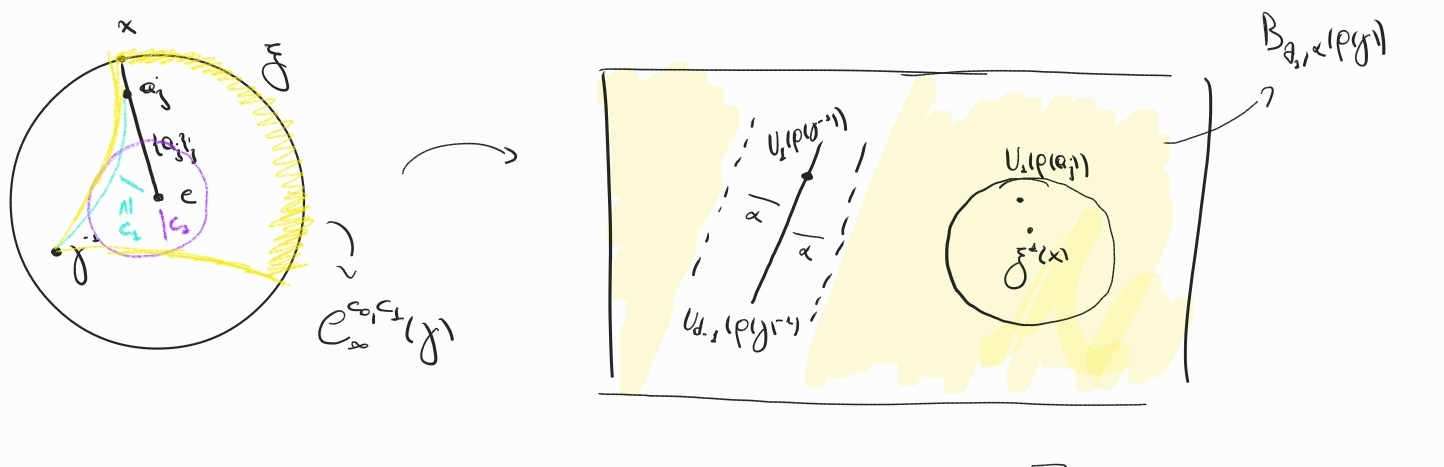
\includegraphics[width=0.8\textwidth]{cone.jpg}
\end{figure}
\section{Proof of bound}
We are now ready to prove the upper bound of the Hausdorff dimension of the limit set by formalizing the proof strategy outlined in the beginning of this chapter.
\begin{lemma}[Upper bound for dimension]\label{lem:upper_bound}
Let $\rho: \Gamma \to \SL(d, \mathbb R)$ be a projective Anosov representation. 
Then:
\[
    \dim_{\mathcal H}(\xi^1 (\partial \Gamma) ) \leq h_{\rho(\Gamma)}(F).
\]
\end{lemma}

\begin{proof}[Proof of \cref{lem:upper_bound}]
Let $p \in \llbracket 2, d \rrbracket$.
Then using \cref{prop:basin_covering}, \cref{lem:boundary_covering}, and \cref{lem:ellipsoid_covering} we have that for $T>0$ large enough, $\xi^1(\partial \Gamma)$ is covered by the family
\[
    \mathcal U_T = \left\{ \rho(\gamma) B_{\alpha_1, \alpha}(\rho(\gamma)) : |\gamma| = T \right\},
\]
and that each basin $\rho(\gamma) B_{\alpha_1, \alpha}(\rho(\gamma))$ is in turn covered by
\[
    2^{p-2} \cdot \frac{\sigma_2(g) \cdots \sigma_{p-1}(g)}{\sigma_p(g)^{p-2}}
\]
many balls of radius
\[
    \sqrt{d-1} \frac{1}{\sin \alpha} \frac{\sigma_p(g)}{\sigma_1(g)}.
\]
By the definition of the Hausdorff measure, for $s \geq 0$:
\begin{align*}
    \mathcal H^s(\xi^1(\partial \Gamma)) &\leq
    \sum_{|\gamma| = T}
        2^{p-2} \cdot 
        \frac{\sigma_2(\rho(\gamma))}{\sigma_1(\rho(\gamma))} \cdots 
            \frac{\sigma_{p-1}(\rho(\gamma))}{\sigma_1(\rho(\gamma))}
        \left(
            \frac{\sigma_p(\rho(\gamma))}{\sigma_1(\rho(\gamma))}
        \right)^{-(p-2)}
        \left(
            \sqrt{d-1} \frac{1}{\sin \alpha} \frac{\sigma_p(\rho(\gamma))}{\sigma_1(\rho(\gamma))}
        \right)^s =\\
        &=
        2^{p-2} \cdot \left( \frac{\sqrt{d-1}}{\sin \alpha}\right)^s  
        \sum_{|\gamma| = T} 
        \frac{\sigma_2(\rho(\gamma))}{\sigma_1(\rho(\gamma))} \cdots 
            \frac{\sigma_{p-1}(\rho(\gamma))}{\sigma_1(\rho(\gamma))}
        \left(
            \frac{\sigma_p(\rho(\gamma))}{\sigma_1(\rho(\gamma))}
        \right)^{s-(p-2)} =\\
        &=
        2^{p-2} \cdot \left( \frac{\sqrt{d-1}}{\sin \alpha}\right)^s  
        \sum_{|\gamma| = T}
        e^{-\left( \alpha_{1 2} + \ldots + \alpha_{1 (p-1)} + (s - (p-2))\alpha_{1 p} \right)\rho(\gamma)}\\
        &=
        2^{p-2} \cdot \left( \frac{\sqrt{d-1}}{\sin \alpha}\right)^s  
        \sum_{|\gamma| = T}
        e^{-\Psi_s^p(\rho(\gamma))}
\end{align*}
and thus
\begin{align*}
    \mathcal H^s(\xi^1(\partial \Gamma)) \leq
    2^{p-2} \cdot \left( \frac{\sqrt{d-1}}{\sin \alpha}\right)^s
    \sum_{|\gamma| = T}
    e^{-\max_p \Psi_s^p(\rho(\gamma)) }\lesssim \sum_{|\gamma| = T} e^{-F_s(\rho(\gamma))}.
\end{align*}
To see that the above implies the upper bound, consider some $s > h_{\rho(\Gamma)}(F)$.
By the definition of the Falconer dimension, this implies that the Dirichlet series corresponding to the Falconer functional converges:
\[
    \sum_{\gamma \in \Gamma} e^{-F_s(\rho(\gamma))} < \infty
\]
and in particular
\[
    \mathcal H^s(\xi^1(\partial \Gamma)) \leq 
    \lim_{T \to \infty} \sum_{|\gamma| = T} e^{-F_s(\rho(\gamma))} = 0.
\]
\end{proof}

Looking again at the proof above, one could wonder whether the cover of the ellipsoid with axes $\beta_2, \cdots, \beta_d$ by balls of radius $\sqrt{d-1} \beta_p$ is optimal, in the sense that it gives the smallest Hausdorff content.
To show that this is the case, consider the cover by balls of radius $r>0$. 
This yields bounds of the form $\mathcal H^s(\xi_\rho^1(\partial \Gamma)) \lesssim \Phi_{r,s}$, where
\[
\Phi_{r,s} = \begin{cases}
    \sum_{|\gamma| = T} r^s, \text{ for } r > \beta_2\\
    \sum_{|\gamma| = T}  \frac{\beta_2 \cdots \beta_{p-1}}{r^{p-2}}  r^s, \text{ for } \beta_{p-1} < r < \beta_p, p \in \llbracket 3, d \rrbracket\\
    \vdots\\
    \sum_{|\gamma| = T}  \frac{\beta_2 \cdots \beta_{d}}{r^{d-1}} r^s, \text{ for } 0 < r < \beta_d.
\end{cases}
\]
The opimality of $r = \beta_p$ can be seen that for $s \in [0,1], \Phi_{r,s}$ is increasing in $[\beta_2, \infty]$, and decreasing in $[0, \beta_2]$, so it is minimized as a function of $r$ for $r = \beta_2$, and thus gives the optimal Hausdroff content when $s \in [0,1]$.
Proceeding similarly, we see that the analogue holds for each of the other intervals as well.

\chapter{Lower bound}\label{ch:lower_bound}
In this chapter we will be bounding the Hausdorff dimension of the limit set from below by the Falconer dimension.
Combining with the reverse inequality obtained in \cref{ch:upper_bound}, this will yield the main result of the thesis:
\begin{reptheorem}{thm:main}
    Let $\rho: \Gamma \to \SL(d, \mathbb R)$ be a Zariski-dense, projective Anosov representation such that $\xi^1_\rho(\partial \Gamma)$ is a Lipschitz submanifold of $\mathbb P(\mathbb R^d)$ of dimension $d_\rho$.
    Then the dimension of the limit set $\xi_\rho^1(\partial \Gamma)$ equals the Falconer dimension of $\rho$:
    \[
        \dim \xi_\rho^1(\partial \Gamma) = h_{\rho(\Gamma)}(F)
    \]
    where $F_s(a) = \max \{ \Psi_s^p(a) : p \in \llbracket 2, d \rrbracket\}$ is the Falconer functional.
\end{reptheorem}
As can be seen from the statement, the lower bound to the dimension will need two more assumptions on the representation: its limit set needs to be a Lipschitz submanifold of the projective dspace and the image needs to be Zariski-dense in $\SL(d, \mathbb R)$.
While the first assumption appears in \cite{pozzetti_anosov_2023} as well, the second one does not, and replaces the assumption that the representation is strongly irreducible.
The reason for this change is that in \cite{pozzetti_anosov_2023} the authors suggest that strong irreducibility of the representation implies that Patterson--Sullivan measures do not admit annihilators of full measure.
However, this is not true, as we show in \cref{ch:no_zariski_density}, where we also discuss further ways to circumvent this issue.

In \cref{sec:busemann} we give the necessary definitions due to \cite{quint2002mesures} that generalise the Busemann cocycle and Patterson--Sullivan measures to Lie groups of higher rank and flag spaces.
Using these, we outline the strategy for the proof of \cref{thm:main} in \cref{sec:ProofStrategy}, which is given in full in \cref{sec:main_thm_proof}.
In \cref{sec:MeasureExistence}, we show that there exists a Patterson--Sullivan measure with the properties that we need. 

\section{Busemann cocyle and Patterson--Sullivan measures}\label{sec:busemann}
We denote with $\Pi$ the set of simple positive roots, and for $\Theta \subseteq \Pi$ we consider the Levi-Anosov subspace of $\mathfrak a$
\[
    \mathfrak a_\Theta = \bigcap_{\alpha \notin \Theta} \ker \alpha,
\]
which in particular admits $\{ \omega_{\alpha_i} : \alpha_i \in \Theta \}$ as a basis.
\begin{definition}\index{Busemann cocycle}
    Let $\Theta \subseteq \Pi$. We define the Busemann cocycle
    \[
    b : \PSL(d, \mathbb R) \times \mathcal F_\Theta \to \mathfrak a_\Theta
    \]
    as the unique element $b(g, k P_\Theta) \in \mathfrak a_\Theta$ such that
    \[
    g k \in K e^{b(g, k P_\Theta)} N.
    \]
    \todo{Correct the definition of the Busemann cocycle\\
    (see \cite{quint2002mesures} Lemme 6.1)\\
    Then add proof for \cref{lem:busemann_weight}}
    where $N = \{ n \in \SL(d, \mathbb R) : n_{ij} = 0 \text{ for } i > j, n_{ii} = 1 \text{ for all } i \}$ is the unipotent group of upper subgroup of upper triangular matrices with $1$s on the diagonal, and $P_\Theta$ is the parabolic subgroup of $\PSL(d, \mathbb R)$ corresponding to $\Theta$, i.e.\ $\mathcal F_\Theta = \PSL(d, \mathbb R)/P_\Theta$.
\end{definition}
\begin{lemma}\label{lem:busemann_weight}
For $y \in \mathcal F_\Theta(\mathbb R^d)$ we have    
\[
    \omega_{\alpha_i}(b_\Theta(g, x)) =
    \log \frac{\| g v_1 \wedge \cdots g v_i \|}{ \| v_1 \wedge \cdots v_i \| }
    \text{ for all } \alpha_i \in \Theta
\]
for any basis $v_1, \ldots, v_i$ of $x^i \in \mathcal G_i(\mathbb R^d)$, where $\| \cdot \|$ denotes the norm on $\bigwedge^i \mathbb R^d$ induced by the euclidean inner product on $\mathbb R^d$, 
i.e.\ $ \langle v_1 \wedge \cdots \wedge v_k, w_1 \wedge \cdots \wedge w_k \rangle := \det(\langle v_i, w_j \rangle)$.
\end{lemma}


\begin{definition}
    We define
    \[
    \Lambda^k : \SL(d, \mathbb R) \to \SL(\Lambda^k \mathbb R^d), \quad
    \Lambda^k : \mathcal G_k(\mathbb R^d) \to \mathbb P(\Lambda^k \mathbb R^d)
    \]
    as
    \[
    \Lambda^k(g)(v_1 \wedge \cdots \wedge v_k) = g v_1 \wedge \cdots \wedge g v_k,\quad
    \Lambda^k(\mathbb R v_1 \oplus \cdots \mathbb R v_k) =  v_1 \wedge \cdots \wedge v_k
    \]
\end{definition}
\begin{lemma}
    Let $g \in \SL(d, \mathbb R), \alpha > 0$ and $k \in \llbracket 2, d \rrbracket$.
    \begin{enumerate}[label=(\roman*)]
        \item $\omega_1(a(\Lambda^k g)) = \omega_k(a(g))$ and $\omega_1(b(\Lambda^k g, \Lambda^k y)) = \omega_k(b(g, y))$.
        \item There exists some $\alpha' > 0$ independent of $g$ such that $\Lambda^k B_{{\sf a}_k, \alpha}(\Lambda^k g) \subseteq B_{{\sf a}_1, \alpha'}(\Lambda^k g)$.
    \end{enumerate}
\end{lemma}
\begin{proof}
    \begin{enumerate}[label=(\roman*)]
        \item Follows from the definitions of the fundamental weights and the Cartan projection.
        \item Let $g = k_g e^{a(g)} l_g$ be the Cartan decomposition of $g$.
        Then using the definitions of the respective subspaces:
        \begin{align*}
        U_{d-k}(g^{-1}l_g^{-1}) &= \mathbb R e_{k+1} \oplus \cdots \oplus \mathbb R e_d\\
        x_0 := U_{d-1}(\Lambda^k g ^{-1} l_g^{-1}) &= \bigoplus_{\substack{i_1 < \cdots < i_k\\(i_1, \cdots, i_k) \neq (1, \cdots, k)}}\mathbb R e_{i_1} \oplus \cdots \oplus \mathbb R e_{i_k}
        \end{align*}
        The first equality implies that
        \[
        y \in B_{{\sf a}_k, \alpha}(g) \Leftrightarrow l_g y \in B_{{\sf a}_k, \alpha}(g l_g^{-1}) = B_{{\sf a}_k, \alpha}(\mathrm{Id}),
        \]
        so for every $y \in B_{{\sf a}_k, \alpha}(g)$ we have that 
        \[
        l_g y = l U_k(\mathrm{Id}) \text{ for some } l \in L
        \]
        where
        \[
        L = \left\{ l \in \SO(d, \mathbb R) : l U_k(\mathrm{Id}) \in B_{{\sf a}_k, \alpha}(\mathrm{Id}) \right\}.
        \]
        Note that $L$ is compact, being a closed subset of a compact group.
        Moreover, the fact that $\Lambda^k(y) \not \in \U_{d-1}(\Lambda^k g^{-1})$ implies that
        \begin{align*}
            0 < \angle(\Lambda^k(y), \U_{d-1}(\Lambda^k g^{-1})) =
            \angle(\Lambda^k(l_g y), \U_{d-1}(\Lambda^k g^{-1} l_g^{-1})) = \angle(\Lambda^k(l) \U_{k}(\mathrm{Id}), x_0)
        \end{align*}
        The right-hand side is in the image of the compact set $L$ under a continuous map, so it is bounded below by a positive number $\alpha' >0$.
        \item Follows from the definition of the Cartan projection and the Busemann cocycle.
    \end{enumerate}
\end{proof}
\begin{definition}\index{Patterson--Sullivan measure}
    For a discrete subgroup $H < \PSL(d, \mathbb R), \phi \in (\alpha_\Theta)^*$,
    an $(H, \phi)$-Patterson--Sullivan measure on $\mathcal F_\Theta$ is a finite Radon measure $\mu$ such that for every $h \in H$
    \[
        \frac{\d h_* \mu}{\d\mu}(x) = e^{-\phi(b_\Theta(h^{-1},x))}, \text{ for all } x \in \mathcal F_\Theta(\mathbb R^d).
    \]
\end{definition}

\begin{lemma}\label{lem:busemann}
Let $\alpha > 0, \Theta \subseteq \Pi$.
There exists $K = K(\alpha) > 0$ such that for each $g \in \SL(d, \mathbb R), \sf{a_i} \in \Theta, y \in B_{\Theta, \alpha}(g), \phi \in \mathfrak a_\Theta$
\[
    |\phi (a(g) - b(g, y))| \leq K.
\]
\end{lemma}\begin{proof}
We begin by noting that it suffices to consider the case where $\phi = {\sf a}_k$
for ${\sf a}_k \in \Theta$, since $\{ \omega_i \}_{{\sf a}_i \in \Theta} $ 
is a basis for $\mathfrak a_\Theta^*$.

We first consider the case where $k=1$.
We recall that the first component of the Cartan projection coincides with the spectral norm of $g$, i.e.
\[
a_1(g) = \log \sup_{v \neq 0} \frac{\| g v\|}{\|v\|} = \log \|g k_2^{-1} e_1 \|
\] 
where $g = k_1 e^{a(g)} k_2$ is the Cartan decomposition of $g$.
Let $v = v_1 k_2^{-1} e_1 + \cdots + v_d k_2^{-1} e_d \in \mathbb R^d$ be such that $\|v\| = 1$ and $y = \mathbb R v$, we have

\begin{align*}
    |\omega_1(a(g) - b(g, y))| &=
    |\log \|g k_2^{-1} e_1 \| - \log \|g v \| | =\\
    &= |\log |e^{a_1(g)}| - \log \| e^{a_1(g)} v_1 k_1 e_1 + \cdots + e^{a_d(g)} v_d k_1 e_d \| | =\\
    &= \left| \log \left\| v_1 k_1 e_1 + e^{-{\sf a}_{12}(g)} v_2 k_1 e_2 + \cdots
    +  e^{-{\sf a}_{1d}(g)} v_d k_1 e_d \right\| \right| \leq\\
    &\leq |\log |v_1| | = \left| \log \sin( \angle(v, U_{d-1}(g^{-1}))) \right| \leq \left| \log \sin \alpha \right|.
\end{align*}

For the case where $\Theta = \{ {\sf a}_k \}$, we consider $\alpha' > 0$ such that
\[
\Lambda^k (B_{{\sf a}_k, \alpha}(g)) \subseteq B_{{\sf a}_k, \alpha'}(\Lambda^k g)
\]
Then using the case $k=1$ we have that
\begin{align*}
    |\omega_k(a(g) - b(g, y))| &=
    |\omega_1(a(\Lambda^k g) - b(\Lambda^k g, \Lambda^k y))| \leq \left| \log \sin \alpha' \right| .
\end{align*}
\end{proof}

\section{Proof strategy}\label{sec:ProofStrategy}
Denoting with $d_\rho = \dim_{\mathcal H} \xi_\rho^1(\partial \Gamma)$ the Hausdorff  dimension of the limit set, we shall outline how to obtain its lower bound by the Falconer dimension
\[
    d_\rho \geq h_{\rho(\Gamma)}(F).
\]

First we recall that $F_s(a) = \max \{ \Psi_s^p(a) : p \in \llbracket 2, d \rrbracket\}$,
so the lower bound will follow once we have shown that
$$d_\rho \geq h_{\rho(\Gamma)}(\Psi^{d_\rho + 1}),$$
since $h_{\rho(\Gamma)}(F) \leq h_{\rho(\Gamma)}(\Psi^{d_\rho + 1})$.

But in \cref{lem:functional_relations}, we showed that $\frac{s}{d_\rho} J_{d_\rho}^u \leq \Psi_{s+d_\rho}^{d_\rho + 1}$, so the above bound will follow as soon as we have shown that
\begin{equation}\label{eq:JacobianBound}
    h_{\rho(\Gamma)}(J_{d_\rho}) \leq 1.\tag{LB}
\end{equation}
which will be obtained using the method of Patterson--Sullivan-Quint.
To apply the latter, apart from showing the existance of a $(J_{d_\rho}^u, \rho)$-Patterson--Sullivan measure $\mu$, we will also need to show that there exists a collection of open sets $\{U_\gamma\}_\gamma \in \Gamma$ such that
\begin{align*}\label{eq:GoodMeasure}
    \mu(U_\gamma) \sim e^{-J_{d_\rho}^u(a(\rho(\gamma)))} \text{ and } 
    M \equaldef \sup_{n \in \mathbb N}
    \max
    \left\{\sharp A : A \subseteq \Gamma_n,  \bigcap_{\gamma \in A}U_\gamma \neq \emptyset \right\} < \infty\tag{MP}
\end{align*}
where $\Gamma_n = \{ \gamma \in \Gamma : |\gamma| = n \} $.
For the proof of the existence of a $(J_{d_\rho}^u, \rho)$-Patterson--Sullivan measure that satisfies the property (\ref{eq:GoodMeasure}) we refer to \cref{sec:MeasureExistence}, noting that the Zariski-density assumption is necessary only for the equivalence appearing on the left hand side of \cref{eq:GoodMeasure}.
Assuming that for the time being, below we outline the Patterson--Sullivan-Quint method of obtaining \cref{eq:JacobianBound}.

Indeed, we first obtain the uniform in $n$ bound:
\begin{align*}
    \sum_{\gamma \in \Gamma_n}
    e^{-J_{d_\rho}^u(a(\rho(\gamma)))} \lesssim
    \sum_{\gamma \in \Gamma_n}
    \mu(U_\gamma) \leq \frac{1}{M} \mu(\mathcal F_\Theta(\mathbb R^d)) < \infty
\end{align*}
along with the bound implied by the Anosov property of $\rho$:
\begin{align*}
J_{d_\rho}(a(\rho(\gamma))) \geq \mathsf a_{12} (a(\rho(\gamma))) \geq C|\gamma| - b
\end{align*}
to conclude that
\begin{align*}
\sum_{\gamma \in \Gamma} e^{-(s+1)J^u_{d_\rho}(a(\rho(\gamma)))} &=
\sum_{n\geq 0} \sum_{\gamma \in \Gamma_n} e^{-s J^u_{d_\rho}(a(\rho(\gamma)))}
    e^{-J^u_{d_\rho}(a(\rho(\gamma)))} \lesssim
\sum_{n\geq 0} e^{-s(Cn - b)} < \infty
\end{align*}
which holds for any $s>0$, and thus \cref{eq:JacobianBound} holds.

\section{Existence of Patterson--Sullivan measure}\label{sec:MeasureExistence}
Let $\rho:\Gamma \to \SL(d, \mathbb R)$ be a projective Anosov representation such that $\xi^1_\rho(\partial \Gamma)$ is a Lipschitz submanifold of dimension $d_\rho$.
A naive approach would be to attempt to construct a Patterson--Sullivan measure over the limit set $\xi^1_\rho(\partial \Gamma)$.
However, complications can arise in the Lipschitz regularity case, because the limit set does not admit a well-defined tangent space at every point.
To overcome this difficulty, proceed as follows.
To almost every $\xi \in \xi_\rho^1(\partial \Gamma)$, we have a well-defined tangent space $T_\xi \xi_\rho^1(\partial \Gamma)$.
The latter, being a subspace of the tangent space $T_\xi(\mathbb P(\mathbb R^d))$ to the projective space $\mathbb P(\mathbb R^d)$, can be seen as the projectivisation (or a hyperplane) of a subspace of $\mathbb R^d$.
In this way we can associate to almost every $\xi \in \xi_\rho^1(\partial \Gamma)$ an element of the flag space $\mathcal F_{1, d_\rho + 1}(\mathbb R^d)$, thus defining a measurable section $\zeta_\rho$.
Restricting the density over the flag space defined in \cref{sec:measures_and_densities}, we obtain an almost every where defined density
\[
    \xi \mapsto |\Omega_{\zeta_\rho(\xi)}|.
\]

The following is \cite[Proposition 6.4]{pozzetti_anosov_2023}:
\begin{proposition}\label{prop:PSMeasureExists}
    Let $\rho: \Gamma \to \SL(d, \mathbb R)$ be a projective Anosov representation, and assume that that $\xi^1_\rho(\partial \Gamma)$ is a Lipschitz submanifold of dimension $d_\rho$.
    Then there exists a $(\rho(\Gamma), J_{d_\rho}^u)$-Patterson--Sullivan measure on $\mathcal F_{1,d_\rho + 1}(\mathbb R^d)$, which is supported on the image of a $\rho$-equivariant measurable section
    \[
    \zeta_\rho: \xi_\rho^1(\partial \Gamma) \to \mathcal F_{1, d_\rho + 1}(\mathbb R^d)
    \]
    of the projection $\mathrm{pr}_1: \mathcal F_{1, d_\rho + 1}(\mathbb R^d) \to \mathbb P(\mathbb R^d)$.
\end{proposition}\todo{Why do we construct a measure over $\mathcal F_{1,d_\rho + 1}(\mathbb R^d)$ and not the limit set? We had talked about it but I forgot.}
\todo{Straighten out this. Does it make sense for $\Omega_{l, V}$ to be an a.e.\ defined density?}
\begin{proof}
    By Rademacher's theorem, $\xi^1_\rho(\partial \Gamma)$ has a well-defined Lebesgue measure class, and Lebesgue-almost every $\xi^1_\rho(x) \in \xi^1_\rho(\partial \Gamma)$ admits a well-defined tangent space $T_{\xi^1_\rho(x)} \xi^1_\rho(\partial \Gamma)$.
    Considering such a $\xi^1_\rho(x)$ we let
    \[
        \pi : \hom(\xi^1_\rho(x), \mathbb R^d) \to \hom(\xi^1_\rho(x), \mathbb R^d/\xi^1_\rho(x)) \simeq T_{\xi^1_\rho(x)} \mathbb P(\mathbb R^d),
    \]
    and
    \[
        x^{d_\rho + 1} = \pi^{-1} (T_{\xi^1_\rho(x)} \xi^1_\rho(\partial \Gamma)) \xi^1_\rho(x) \in 
        \mathcal G_{d_\rho + 1} (\mathbb R^d).
    \]
    The calculation of the dimension follows from the rank-nullity theorem on 
    $\pi$ restricted to  $\pi^{-1}(T_{\xi_\rho^1(x)} \xi_\rho^1(\partial_\Gamma))$ 
    and the fact that  
    $\xi_\rho^1(\partial \Gamma) \leq \pi^{-1}(T_{\xi_\rho^1(x)} \xi_\rho^1(\partial_\Gamma)) $. 
    Then \cref{prop:grassmanian_tangent_flags} implies that
    \[
        T_{\xi^1_\rho(x)} \xi^1_\rho(\partial \Gamma) = 
        \hom(\xi^1_\rho(x), x^{d_\rho + 1} / \xi^1_\rho(x)),
    \]
    In this notation, we shall define (Lebesgue-almost everywhere) the map
    \begin{align*}
        \zeta_\rho: \xi_\rho^1(\partial \Gamma) \to \mathcal F_{1, d_\rho + 1} (R^d), \quad 
        \zeta_\rho(\xi_\rho^1(x)) = (\xi_\rho^1(x), x^{d_\rho + 1}).
    \end{align*}
    which is a section in the sense that the projection $\mathrm{pr}_1: \mathcal F_{1, d_\rho + 1} \to \mathbb P(\mathbb R^d)$ to the first coordinate satisfies $\mathrm{pr}_1 \circ \zeta_\rho = \mathrm{Id}$.
    Moreover, it is $\rho(\Gamma)$ equivariant, since for $\gamma \in \Gamma$ we have
    \begin{align*}
        \rho(\gamma) \zeta_\rho(\xi_\rho^1(x)) &=
         \left( \rho(\gamma) \xi_\rho^1(x), 
            \rho(\gamma) \pi^{-1}(T_{\xi_\rho^1(x)} \xi_\rho^1(\partial \Gamma)) \right) =\\
        &= \left( \rho(\gamma) \xi_\rho^1(x), 
        \rho(\gamma) \pi^{-1}(T_{\xi_\rho^1(x)} \xi_\rho^1(\partial \Gamma)) \rho(\gamma)^{-1} \rho(\gamma) \xi_\rho^1(x) \right) =\\
        &= \left( \rho(\gamma) \xi_\rho^1(x), 
           \pi^{-1}(\rho(\gamma) T_{\xi_\rho^1(x)} \xi_\rho^1(\partial \Gamma)) \right) =\\
        &= \left( \rho(\gamma) \xi_\rho^1(x), 
        \pi^{-1}(T_{\rho(\gamma) \xi_\rho^1(x)} \xi_\rho^1(\partial \Gamma)) \right) =\\
        &= \zeta_\rho(\rho(\gamma) \xi_\rho^1(x)) = 
        \zeta_\rho( \xi_\rho^1(\gamma x)).
    \end{align*}
    \todo{Why is the section measurable?}
    We now define the non-negative density on $\xi_\rho^1(\partial \Gamma)$
    \[
        \mu_{\xi_\rho^1(x)} = |\Omega_{\zeta_\rho(\xi_\rho^1(x))}|
    \]
    which satisfies
    \[
        \frac{\d \rho(\gamma)_*\mu}{\d\mu}(\xi) = \frac{\d (\rho(\gamma)^{-1})^*\mu}{\d\mu}(\xi) =
        e^{-J^u_{d_\rho + 1}(b_\Theta(\rho(\gamma)^{-1}, \zeta_\rho(x)))},
    \]
    where the term on the left-hand side involves measures, the term between the two equalities involves densities, and $\Theta = \{1, d_\rho + 1\}$.
    The first equality holds for any density and its respective measure, while for the second one we consider $\phi_1, \ldots, \phi_{d_\rho} \in T_{\xi_\rho^1(x)}\xi_\rho^1(\partial \Gamma)$ and calculate:
    \begin{align*}
        &(\rho(\gamma)^*\mu)_{\xi_\rho^1(x)} (\phi_1, \ldots, \phi_{d_\rho})\\
        &=
        \mu_{\rho(\gamma)\xi_\rho^1(x)} (\rho(\gamma)\phi_1\rho(\gamma)^{-1}, \ldots, \rho(\gamma)\phi_{d_\rho} \rho(\gamma)^{-1}) \\
        &=
        \frac{\|\rho(\gamma) \xi_\rho^1(x) \wedge \rho(\gamma) \phi_1(\xi_\rho^1(x)) \wedge \cdots \wedge \rho(\gamma) \phi_{d_\rho}(\xi_\rho^1(x))\|}
        {\| \rho(\gamma) \xi_\rho^1(x) \|^{d_\rho + 1}} \\
        &=
        \frac{\|\rho(\gamma) \xi_\rho^1(x) \wedge \rho(\gamma) \phi_1(\xi_\rho^1(x)) \wedge \cdots \wedge \rho(\gamma) \phi_{d_\rho}(\xi_\rho^1(x))\|}
        {\|\xi_\rho^1(x) \wedge \phi_1(\xi_\rho^1(x)) \wedge \cdots \wedge \phi_{d_\rho}(\xi_\rho^1(x))\|} \\
        &\quad \cdot
        \frac{\|\xi_\rho^1(x) \wedge \phi_1(\xi_\rho^1(x)) \wedge \cdots \wedge \phi_{d_\rho}(\xi_\rho^1(x))\|}
        {\|\rho(\gamma) \xi_\rho^1(x)\|^{d_\rho+1}}\cdot
        \frac{\| \rho(\gamma)\xi_\rho^1(x)\|^{d_\rho+1}}{\|\xi_\rho^1(x)\|^{d_\rho+1}} \\
         &=
         e^{\omega_{d_\rho}(b_\Theta(\rho(\gamma), \zeta_\rho(\xi_\rho^1(x))))} \cdot
         \mu_{\xi_\rho^1(x)}(\phi_1, \ldots, \phi_{d_\rho}) \\
         &\quad \cdot
         e^{-(d_\rho+1)\omega_1(b_\Theta(\rho(\gamma), \zeta_\rho(\xi_\rho^1(x))))} \\
         &=
         e^{-J_{d_\rho}^u(b_\Theta(\rho(\gamma)^{-1}, \zeta_\rho(\xi_\rho^1(x))))} \mu_{\xi_\rho^1(x)}(\phi_1, \ldots, \phi_{d_\rho}).
    \end{align*}
    
    Finally, we let $\nu = {\zeta_\rho}_* \mu$, which is the wanted Patterson--Sullivan measure on $\mathcal F_{1, d_\rho + 1} (\mathbb R^d)$, since for $f \in C_c(\mathcal F_{1, d_\rho + 1} (\mathbb R^d))$:
    \begin{align*}
        \int_{\mathcal F_{1, d_\rho + 1} (\mathbb R^d)} f \d(\rho(\gamma)_* {\zeta_\rho}_* \mu) &=
        \int_{\xi_\rho^1(\partial \Gamma)} f \circ \rho(\gamma) \circ \zeta_\rho \d \mu =
        \int_{\xi_\rho^1(\partial \Gamma)} f \circ \zeta_\rho \circ \rho(\gamma) \d \mu =\\
        &=
        \int_{\xi_\rho^1(\partial \Gamma)} f \circ \zeta_\rho(\xi_\rho^1(x)) e^{-J_{d_\rho}^u(b_\Theta(\rho(\gamma)^{-1}, \zeta_\rho(\xi_\rho^1(x)))} \d \mu(\xi_\rho^1(x)) =\\
        &=
        \int_{\mathcal F_{1, d_\rho + 1} (\mathbb R^d)} 
        f(y) e^{-J_{d_\rho}^u(b_\Theta(\rho(\gamma)^{-1}, y)} \d ({\zeta_\rho}_*\mu)(y)
    \end{align*}
\end{proof}

Our next goal is to find a collection of sets $(U_\gamma)_{\gamma \in \Gamma}$ such that $e^{-J^u_{d_\rho}(a(\rho(\gamma)))} \lesssim \mu(U_\gamma)$ and whose sets do not intersect a lot.
In the next lemma we define this collection and show its intersection property.
It should be regarded as an analog of \cref{lem:boundary_covering} and \cref{prop:shadows} to arbitrary flag varieties, and relies only on the Anosov property of $\rho$, and the fact that $\zeta_\rho$ is a section of $\pi_{\sf a_1}: \mathcal F_{1, d_{\rho,\Gamma}+1}(\mathbb R^d) \to \mathbb P(\mathbb R^d)$.
\begin{lemma}\label{lem:boundary_covering_higher}
Let $\rho: \Gamma \to \SL(d, \mathbb R)$ be projective Anosov and $\Theta = \{ {\sf a}_1, {\sf a}_{d_{\rho}}\} \subseteq \Pi$.
Then for $\alpha > 0$ small enough, there exists some $C, T_0 > 0$ such that for all $T \geq T_0$ the family
\[
    \mathcal U_T = \left\{ \rho(\gamma) B_{\Theta, \alpha}(\rho(\gamma)) : |\gamma| = T \right\}
\]
is a collection of open subsets of $\mathcal F_\Theta(\mathbb R^d)$ such that every $\zeta_\rho(\xi^1_\rho(x))$ is contained in at most $C$ many sets in $\mathcal U_T$.
\end{lemma}
\begin{proof}
Suppose $\zeta_\rho(\xi^1_\rho(x)) \in \rho(\gamma) B_{\Theta, \alpha}(\rho(\gamma)) \cap \rho(\eta) B_{\Theta, \alpha}(\rho(\eta))$ for some $\gamma, \eta \in \Gamma_T$.
Then $\xi_\rho^1(x) \in \rho(\gamma) B_{{\sf a}_1, \alpha}(\rho(\gamma)) \cap \rho(\eta) B_{{\sf a}_1, \alpha}(\rho(\eta))$.
But using \cref{prop:shadows} we have that
\begin{align*}
    x &\in (\xi_\rho^1)^{-1}(\rho(\gamma) B_{{\sf a}_1, \alpha}(\rho(\gamma)) \cap \rho(\eta) B_{{\sf a}_1, \alpha}(\rho(\eta))) =\\
    &= \gamma(\xi_\rho^1)^{-1}(B_{{\sf a}_1, \alpha}(\rho(\gamma))) \cap \eta (\xi_\rho^1)^{-1}(B_{{\sf a}_1, \alpha}(\rho(\eta))) \subseteq\\
    &\subseteq \gamma C_{c_0, c_1}(\gamma) \cap \eta C_{c_0, c_1}(\eta).
\end{align*}
Thus $x$ is represented by $(c_0, c_1)$-quasi-geodesic rays $(a_j)_0^\infty, (b_j)_0^\infty $, that start from $e$ and pass from $\gamma$ and $\eta$ respectively.
By Morse's lemma, we know that there exists some geodesic ray starting from $e$ and some $A > 0$ depending only on $c_0, c_1$ and the hyperbolicity constant of $\Gamma$ such that the Hausdorff distance of the geodesic ray to each of the quasi-geodesics is bounded by $A$. 
Let $\epsilon_0, \epsilon_1$ be two points on the geodesic ray such that $\d(\gamma, \epsilon_0), \d(\eta, \epsilon_1) \leq A$.
Then we have that
\begin{align*}
    \d(\gamma, \eta) &\leq \d(\gamma, \epsilon_0) + \d(\epsilon_0, \epsilon_1) + \d(\epsilon_1, \eta) \leq 
    2A + | |\epsilon_0| - |\epsilon_1|| \leq\\
    &\leq
    2A + | |\epsilon_0| - |\gamma|| + | |\gamma| - |\eta| | + | |\epsilon_1| - |\eta|| \leq 4A.
\end{align*}
In particular, any $\gamma'$ such that $\zeta_\rho(\xi^1_\rho(\gamma'))  \in \xi_\rho^1(\rho(\gamma') B_{\Theta, \alpha}(\rho(\gamma')))$, will lie in a ball of radius $4A$ around $\gamma$.
Since $\Gamma$ is finitely generated, there exists some $C > 0$ such that the ball of radius $4A$ around $\gamma$ contains at most $C$ elements of $\Gamma$.
\end{proof}

To show the equivalence $e^{-J_{d_\rho}^u(a(\rho(\gamma)))} \sim \mu(\rho(\gamma)B_{\Theta, \alpha}(\rho(\gamma))$, aside from the equivariance property of $\mu$, we will also need for it to ``see the whole space of flags $\mathcal F_\Theta(\mathbb R^d)$'' and not just part of it.
To make this more concrete, we introduce the following two definitions from \cite{pozzetti_anosov_2023}.

\begin{definition}
    Let $\Theta \subseteq \Pi$.
    We define the annihilator of an element $y \in \mathcal F_{i \Theta}(\mathbb R^d)$ is the set of partial flags in $\mathcal F_\Theta(\mathbb R^d)$ that are not transverse to $y$, that is:
    \[
        \mathrm{Ann}(y) = \left\{ x \in \mathcal F_{\Theta}(\mathbb R^d) : x^\theta \cap y^{d- \theta} \neq 0 \text{ for some } \theta \in \Theta \right\}.
    \]    
\end{definition}

\begin{definition}\index{irreducible representation!with respect to measure}
    \label{def:mu_irreducible}
Let $\rho: \Gamma \to \SL(d,\mathbb R)$ be a linear representation, $\Theta \subseteq \Pi$ and $\mu$ a $(\rho(\Gamma), \phi)$-Patterson--Sullivan measure over $\mathcal F_\Theta(\mathbb R^d)$.
We say that $\rho$ is $\mu$-irreducible if there is no element in $\mathcal F_{i \Theta}(\mathbb R^d)$, whose annihilator is of full measure, i.e.\ for all $y \in \mathcal F_{i \Theta}(\mathbb R^d)$:
\[
    \mu(\mathrm{Ann}(y)) < \mu(\mathcal F_{\Theta}(\mathbb R^d)).
\]
\end{definition}

The following example will be also the case that is of interest to us in this chapter.
\begin{example}\label{ex:ZariskiDense}
    Let $\rho: \Gamma \to \SL(d,\mathbb R)$ be a linear representation and $\Theta \subseteq \Pi$.
    If $\rho(\Gamma)$ is Zariski-dense in $\SL (d, \mathbb R)$, then $\rho$ is $\mu$-irreducible for any $\rho(\Gamma)$-quasi-invariant measure $\mu$ on $\mathcal F_\Theta(\mathbb R^d)$, and in particular for any $(\rho(\Gamma), \phi)$-Patterson--Sullivan measure.
\end{example}
\begin{proof}
    We will show that the support of $\mu$ is the full space $\mathcal F_\Theta(\mathbb R^d)$.
    Quasi-invariance implies that for all $\rho(\gamma) \in \rho(\Gamma)$
    \[
    \supp \mu = \supp \rho(\gamma)_* \mu = \rho(\gamma) \supp \mu,
    \]
    and thus the support of $\mu$ is $\rho(\Gamma)$-invariant: $\rho(\Gamma) \supp \mu = \rho(\Gamma) \supp \mu$.
    Taking the closure we see that $\supp \mu$ is in fact $\SL(d, \mathbb R)$-invariant and hence contains the whole space $\mathcal F_\Theta(\mathbb R^d)$ because the action of $\SL(d, \mathbb R)$ on the latter is transitive.
\end{proof}

The following proposition shows the reason that we introduce the concept of $\mu$-irredubility.
It allows us to bound the measure of bassins of attraction uniformly from below.
\begin{proposition}\label{prop:irreducibility}
    Let $\rho: \Gamma \to \SL(d,\mathbb R)$ be a linear representation, $\Theta \subseteq \Pi$ and $\mu$ a $(\rho(\Gamma), \phi)$-Patterson--Sullivan measure over $\mathcal F_\Theta(\mathbb R^d)$.
    If $\rho$ is $\mu$-irreducible, then there exist $\alpha, \kappa > 0$ such that $\mu(B_{\Theta, \alpha}(\rho(\gamma))) \geq k$ for all $\gamma \in \Gamma$.
\end{proposition}
\begin{proof}
    If this were not the case, then there would exists a sequence $\alpha_n \searrow 0$ and $\gamma_n \in \Gamma$ such that
    \[
        \mu(B_{\Theta, \alpha_n}(\rho(\gamma))) \leq \frac{1}{n}.
    \]
    Due to the compactness of $\mathcal F_{\Theta} (\mathbb R^d)$, up to considering a subsequence, we may assume that the repelling flags or $\rho(\gamma_n)$ converge to some $\xi \in \mathcal F_{\Theta} (\mathbb R^d)$:
    \[
        (U_{d-i}(\rho(\gamma_n)^{-1}))_{\mathsf a_i \in \Theta} \to \xi
    \]
    
    In that case, the complements $B_{\Theta, \alpha_n}^c(\rho(\gamma_n))$ will converge to the annihilator of $\xi$, in the sense:
    \[
        \limsup_n B_{\Theta, \alpha_n}^c(\rho(\gamma_n)) \subseteq \mathrm{Ann}(\xi).
    \]
    Indeed, let $y\in \limsup_n  B_{\Theta, \alpha_n}^c(\rho(\gamma_n))$ and consider a subsequence $k_n$ such that $y\in B_{\Theta, \alpha_n}^c(\rho(\gamma_{k_n}))$.
    By the very definition of $B_{\Theta, \alpha_n}(\rho(\gamma_n))$, there exists some $p$ such that up to considering a subsequence of $k_n$,
    \[
        \angle (y^p, U_{d-p}(\rho(\gamma_n)^{-1})) \leq \alpha_n
    \]
    holds.
    Taking the limit as $n \to \infty$, we have that $y^p \cap \xi^{d-p} \neq 0$ and hence $y \in \mathrm{Ann(\xi)}$.

    Using a measure-theoretic arguement we conclude that $\mathrm{Ann}(\xi)$ is of full measure
    \[
        \mu(\mathrm{Ann}(\xi)) \geq
        \mu (\limsup_n B_{\Theta, \alpha_n}^c(\rho(\gamma_{k_n})) ) \geq 
        \limsup_n \mu (B_{\Theta, \alpha_n}^c(\rho(\gamma_{k_n}))) =
        \mu(\mathcal F_\Theta (\mathbb R^d)),
    \]
    which contradicts the $\mu$-irreducibility of $\rho$.
\end{proof}
We are now ready to show the equivalence $\mu(\rho(\gamma)B_{\Theta, \alpha}(\rho(\gamma))) \simeq e^{-J^u_{d_\rho}(a(\rho(\gamma)))}$ when the representation $\mu$-irreducible.
\begin{lemma}\label{lem:PSMeasureBounds}
    Let $\rho:\Gamma \to \SL(d, \mathbb R)$ be a representation and $\mu^\phi$ be a ($\rho(\Gamma), \phi$)-Patterson--Sullivan measure.
    If $\rho(\Gamma)$ is $\mu$-irreducible, then there exists some $\alpha_0 > 0$, such that for any $\alpha \in (0, \alpha_0)$, there is some $k = k(\alpha) > 0$ for which
    \[
        \frac{1}{k} e^{-\phi(a(\rho(\gamma)))} 
        \leq 
        \mu^\phi(\rho(\gamma) B_{\Theta, \alpha}(\rho(\gamma))) 
        \leq
        k e^{-\phi(a(\rho(\gamma)))} 
    \]
    for all $\gamma \in \Gamma$. 
\end{lemma}
\begin{proof}
    Let $\alpha_0, k > 0$ be as in the remark preceeding the statement of the lemma.
    As noted in \cref{lem:busemann}, there exists some $K = K(\alpha_0, \phi) > 0$ such that for any $\alpha \in (0, \alpha_0)$ and $y \in B_{\Theta, \alpha}(\rho(\gamma))$:
    \[
        |\phi(a(\rho(\gamma)) - b(\rho(\gamma), y))| \leq K,
    \]
    from which we obtain the upper bound
    \begin{align*}
        \mu^\phi(\rho(\gamma) B_{\Theta, \alpha}(\rho(\gamma))) &=
        (\rho(\gamma^{-1})_*\mu^\phi)(B_{\Theta, \alpha}(\rho(\gamma))) =
        \int_{\mathcal F_\Theta(\mathbb R^d)} e^{-\phi(b(\rho(\gamma), y))} d\mu^\phi(y)\leq\\
        &\leq
        e^{-K} \mu^\phi(\mathcal F_\Theta (\mathbb R^d)) e^{-\phi(a(\rho(\gamma)))}.
    \end{align*}
    
    Similarly we obtain the lower bound.
\end{proof}
\section{Proof of the main theorem}\label{sec:main_thm_proof}
In this section we shall prove the main theorem, which we restate for the reader's convenience:
\begin{theorem}\label{thm:main}
    Let $\rho: \Gamma \to \SL(d, \mathbb R)$ be a Zariski-dense, projective Anosov representation such that $\xi^1_\rho(\partial \Gamma)$ is a Lipschitz submanifold of $\mathbb P(\mathbb R^d)$ of dimension $d_\rho$.
    Then the dimension of the limit set $\xi_\rho^1(\partial \Gamma)$ equals the Falconer dimension of $\rho$:
    \[
        \dim \xi_\rho^1(\partial \Gamma) = h_{\rho(\Gamma)}(F)
    \]
    where $F_s(a) = \max \{ \Psi_s^p(a) : p \in \llbracket 2, d \rrbracket\}$ is the Falconer functional.
\end{theorem}
\begin{proof}
    We have already seen in \cref{lem:upper_bound} that $d_\rho \leq h_{\rho(\Gamma)}(F)$.
    For the opposite inequality, we merely need to piece together the results of the previous sections as outlined in \cref{sec:ProofStrategy}.
    There we have seen that $h_{\rho(\Gamma)}(F) \leq h_{\rho(\Gamma)}(\Psi^{d_\rho + 2})$ since $F_s \geq \Psi_s^{d_\rho + 2}$, so may as well show that $h_{\rho(\Gamma)}(\Psi^{d_\rho + 2}) \leq d_\rho$, i.e.\ that
    \[
        \sum_{\gamma \in \Gamma} e^{-\Psi^{d_\rho + 2}_s(\rho(\gamma))} < \infty
    \]
    for all $s \geq d_\rho$.
    This will follow as soon as we have shown that $h_{\rho(\Gamma)}(J_{d_\rho}) \leq 1$, since $\Psi_s^{d_\rho + 1} \geq \frac{s}{d_\rho} J_{d_\rho}^u$, as we saw in \cref{lem:functional_relations}.
    
    Using the Anosov property of $\rho$ we have that
    \[
    J_{d_\rho}(a(\rho(\gamma))) \geq \mathsf a_{12} (a(\rho(\gamma))) \geq C|\gamma| - b    
    \]
    for certain $C, b > 0$ which when we break up the sum defining the critical exponent into the sum over the sets $\Gamma_T = \{ \gamma \in \Gamma: |\gamma| = T\}$ gives us:
    \begin{align*}
        \sum_{\gamma \in \Gamma} e^{-(s+1)J_{d_\rho}^u(a(\rho(\gamma)))} &=
        \sum_{T \geq 0} \sum_{\gamma \in \Gamma_T} e^{-s J_{d_\rho}^u(a(\rho(\gamma)))}
        e^{-J_{d_\rho}^u(a(\rho(\gamma)))} =\\
        &=
        \sum_{T \geq 0} e^{-s J_{d_\rho}^u(a(\rho(\gamma)))} 
            \sum_{\gamma \in \Gamma_T} e^{-J_{d_\rho}^u(a(\rho(\gamma)))} \leq\\
        &\leq
        \sum_{T \geq 0} e^{-s (C T - b)} 
            \sum_{\gamma \in \Gamma_T} e^{-J_{d_\rho}^u(a(\rho(\gamma)))}\\
    \end{align*}
    
    To obtain a bound on the inner sums that is uniform in $T$, we recall \cref{prop:PSMeasureExists}. 
    There we saw that $\xi^1_\rho(\partial \Gamma)$ being a Lipschitz submanifold of $\mathbb P(\mathbb R^d)$ implies the existence of a $(\rho(\Gamma), J_{d_\rho}^u)$-Patterson--Sullivan measure $\mu$ on $\zeta^1_\rho(\xi^1(\partial \Gamma)) \subseteq \mathcal F_{1, d_\rho + 1}(\mathbb R^d)$.
    By \cref{lem:boundary_covering_higher} we have that for $\alpha > 0$ small enough, there exists some $M, T_0 > 0$ such that for all $T \geq T_0$ the family
    \[
        \mathcal U_T = \left\{ \rho(\gamma) B_{\alpha, \Theta}(\rho(\gamma)) : |\gamma| = T \right\}
    \]
    is an open covering of $\zeta_\rho(\xi^1_\rho(\partial \Gamma))$ for which
    \[
        \max
        \left\{\sharp A : A \subseteq \Gamma_T,  \bigcap_{\gamma \in A}\rho(\gamma)B_{\alpha, \Theta}(\rho(\gamma)) \neq \emptyset \right\} \leq M.
    \]

    But $\mu$ is $\rho(\Gamma)$-quasi-invariant which along with the Zariski-density of $\rho(\Gamma)$ implies that $\rho$ is $\mu$-irreducible, as we have seen in \cref{ex:ZariskiDense}.
    Hence the bound in \cref{lem:PSMeasureBounds} applies and we have that
    \begin{align*}
        \sum_{\gamma \in \Gamma_T} e^{-J_{d_\rho}^u(a(\rho(\gamma)))} &\leq
        \sum_{\gamma \in \Gamma_T} \mu\left(\rho(\gamma) B_{\alpha, \Theta}(\rho(\gamma))\right) \leq\\
        &\leq
        \frac{1}{M} \mu\left(\mathcal F_{1, d_\rho + 1}(\mathbb R^d)\right) < \infty.
    \end{align*}

    
\end{proof}

\chapter{Dropping the Zariski-density assumption}\label{ch:no_zariski_density}
Since many interesting examples of Anosov subgroups are not Zariski-dense, one could certainly argue that the Zariski-density assumption in \cref{thm:main} is not cheap.
The reason that it's needed is that otherwise one can't guarantee that it is $\mu$-irreducible for a Patterson--Sullivan measure $\mu$. 
In fact, Zariski-density is not assumed and takes the place of strong irredubility in \cite{pozzetti_anosov_2023}, where the authors suggest the latter implies $\mu$-irredubility through the following lemma which as we will see below is false.

\begin{lemma}[Lemma 6.8 in \cite{pozzetti_anosov_2023}]\label{lem:irreducibility}
Let $\Gamma$ be a hyperbolic group and $\eta:\Gamma \to \PGL(d, \mathbb R)$ be a strongly irreducible projective Anosov representation such that $\xi_\eta(\partial \Gamma)$ is homeomorphic to $\mathbb S^{d_\rho}$, and which admits a measurable $\eta$-equivariant section
$\zeta: \partial \Gamma \to \mathcal F_{\{ \sf a_1, \sf a_{d_\rho + 1}\}} (\mathbb R^d)$.
Then $\eta$ is $\mu$-irreducible for any $(\eta(\Gamma), \phi)$-Patterson--Sullivan measure $\mu$ on $\zeta(\partial \Gamma) \subseteq \mathcal F_{\{ \sf a_1, \sf a_{d_\rho + 1}\}} (\mathbb R^d)$.
\end{lemma}

For convenience, we recall that a linear representation $\rho: \Gamma \to \GL(d, \mathbb R)$ is strongly irreducible\index{irreducible representation!strongly} if there is no proper $\rho(\Gamma)$-invariant subspace of $\mathbb R^d$,
and it is $\mu$-irreducible if there is no element in $\mathcal F_{i \Theta}(\mathbb R^d)$, whose annihilator is of full measure.

More specifically, in the proof of the preceeiding lemma, the authors argue by contradiction that if the result is not true, then there exists subspaces $W_0 \in \mathcal G_{d-d_\rho - 1}$ and $V \in \mathcal G_{d-d_\rho - 1}$ such that
\[
\eta(\gamma) V \cap W_0 \neq 0
\]
for all $\gamma \in \Gamma$.
Indeed, if this were not the case, then there exist $(W_0, P_0) \in \mathcal F_{{\sf a}_{d-d_\rho - 1}, {\sf a}_{d-1}}$ such that $\mathrm{Ann}(W_0,P_0)$ is of full $\mu$ measure.
In fact, $\eta$-equivariance of $\zeta$ implies that one can choose $W_0, P_0$ such that $P_0 \in \xi^{d-1}_\eta(\partial \Gamma)$, meaning that for $\mu$-almost every $(\xi^1_\eta(x), \zeta(x)^{d_\rho + 1}) \in \zeta(\partial \Gamma)$, we have that $\zeta(x)^{d_\rho + 1} \cap W_0 \neq 0$.
Again using the $\eta$-equivariance of $\zeta$, we have that for all $\gamma \in \Gamma$, the set 
$\left\{ \zeta(x) \in \zeta(\partial \Gamma) : \zeta(x)^{d_\rho + 1} \cap \gamma W_0 \neq 0 \right\}$
is of full measure, which implies that their intersection is non-empty, and we can take $V = \zeta(x)^p$ for any $x \in \partial \Gamma$ such that $\zeta(x)$ lies in this intersection.

Finally to conlude, the authors assert that this contradicts strong irreducibility by using \cite[Proposition 10.3]{labourie_anosov_2006}:
\begin{proposition}[Labourie]\label{prop:labourie}
Let $G \leq \SL(d, \mathbb R)$ be an algebraic group.
If $C \in \mathcal G_{k}(\mathbb R^d), B \in \mathcal G_{d-k}(\mathbb R^d)$ such that
\begin{equation}\label{eq:irreducibility}
    g C \cap B \neq 0 \text{ for all } g \in G,
\end{equation}
then the connected component of $G$ containing the identity element is not irreducible.
\end{proposition}

However, \cref{prop:labourie} and consequently \cref{lem:irreducibility} are false, leaving room for further investigation.
In particular, below we present a direct counterexample to \cref{prop:labourie}, followed by a construction which shows that \cref{eq:irreducibility} does not contradict strong irreducibility, and where the representation $\eta$ is not $\mu$-irreducible, thus disproving \cref{lem:irreducibility}.
Nevertheless, if we proceed to calculate the dimension of the respective limit set and the critical exponent of the Falconer functional, we notice that they coincide and hence do not provide a counterexample to the main result presented in \cite{pozzetti_anosov_2023}, which suggests that the result may still hold at least for certain special cases.

\section{Two counterexamples}\label{sec:two_counterexamples}
We begin by providing a counterexample to \cref{prop:labourie}.
For this, we use the space $\mathbb R^{d,d}$, which we recall to be $\mathbb R^{2d}$ equipped with the bilinear form $\langle x, y \rangle = x_1 y_1 + \cdots + x_d y_d - x_{d+1} y_{d+1} - \cdots y_{2d}$.
\begin{example}
    Let $S \subseteq \mathcal G_d (\mathbb R^{2d})$ to be the set of maximal isotropic subspaces of $\mathbb R^{d,d}$.
    If $d$ is odd, then for any subspaces $V, W$ in the same component of $S$, we have 
    \[
        gV \cap W \neq 0 \text{ for all } g \in \SO(d,d).
    \]
\end{example}
\begin{proof}
    We begin by parametrizing the set $S$ by $\mathrm{O}(d)$.
    For completeness we note that this parametrization is independent of the parity of $d$.
    \[\begin{array}{lll}
        &S \quad &\leftrightarrow \quad \mathrm{O}(d) \\
        &V \quad &\mapsto \quad \mathrm{pr}_2 \circ ({\mathrm{pr}_1}_{|V})^{-1} \\
        &\Gamma(\phi) \quad &\mapsfrom \quad \phi
    \end{array}\]
    where we denote with $\mathrm{pr}_1, \mathrm{pr}_2: \mathbb R^{d,d} \to \mathbb R^d$ the projections to the first and last $d$ coordinates, and $\Gamma(\phi) = \left\{ (x, \phi(x)) : x \in \mathbb R^d\right\}$ the graph of $\phi \in \mathrm{O}(d)$. 
    The left-to-right direction of this correspondence is well-defined because all $V \in S$ are $d$-dimensional and transverse to $\mathbb R^d \oplus 0$ and $0 \oplus \mathbb R^d$.

    For the next step, we will need the assumption that $d$ is odd and we will show that any pair of spaces $V, W$ in the same connected component of $S$ are non-transverse.
    Indeed, note that $\phi, \psi \in \mathrm{O}(d): \Gamma(\phi) \cap \Gamma(\psi) \neq 0$ if and only if $\psi \circ \phi^{-1}$ admits $1$ as an eigenvalue.
    The latter is true when $\det \psi = \det \phi$ or equivalently when $\phi, \psi$ are in the same component of $\mathrm{O}(d)$.

    Under the parametrisation of $S$ via $\mathrm{O}(d)$, the action $SO(d,d) \curvearrowright S$ is $g \cdot \Gamma(\phi) = \Gamma(g \phi g^{-1})$.
    Since $\det (g \phi g^{-1}) = \det (\phi)$, we know that $\SO(d,d)$ preserves each component of $S$.

    To see why $\SO_0(d,d)$ acts irreducibly on $\mathbb R^{d,d}$, we note that $\SO(d) \times \SO(d)$ acts irreducibly on $\mathbb R^{d,d}$ and is contained in $\SO_0(d,d)$.
\end{proof}

After providing a counterexample to \cref{prop:labourie} as above, one could object that this does not necessarily imply that the result of \cref{lem:irreducibility} is false.
For this, one would need to provide another counterexample for \cref{lem:irreducibility} as well, which is the goal of the next pages and is summarised in \cref{prop:irreducibility_countexample}.
Before giving the statement of the latter, we recall that a uniform lattice $\Gamma$ \index{uniform lattice} of a locally compact group $G$ is a discrete subgroup of $G$ that is co-compact, i.e.\ $G/\Gamma$ is compact.

Since we will be working with $\SU(2,1)$ and $\SL(su(2,1))$,we will use different symbols for their Cartan projections to avoid confusion.
We will denote with $\mu: \SU(2,1) \to \mathfrak a^+$ and $a:\SL(\su(2,1)) \to \mathfrak a^+$ the projections of $ \SU(2,1)$ and $\SL(\su(2,1))$ respectively.

\begin{proposition}\label{prop:irreducibility_countexample}
    Let $\Gamma \leq \SU(2,1)$ be a uniform lattice and $\eta: \Gamma \to \SL(\mathfrak{su}(2,1))$ be the restriction of the adjoint representation.
    Then
    \begin{enumerate}[label=(\roman*)]
        \item $\eta$ is strongly irreducible,
        \item $\eta$ is projective Anosov
        \item $\eta$ admits a continuous $\eta$-equivariant section: 
        \begin{align*}
            \zeta: \partial \Gamma &\to \mathcal F_{\{1, 4 \}}(\mathfrak{su}(2,1)) \simeq \mathcal P\\
            x &\mapsto (\xi^1(x), T_{\xi^1(x)} \xi^1(\partial \Gamma)) \simeq (\xi^1(x), (\d_{\xi^1(x)}p)^{-1}(T_{\xi^1(x)}\xi^1(\partial \Gamma))\xi^1(x)).
        \end{align*}
        where $d_{\xi^1(x)}p: \hom( \xi^1(x), \su(2,1)) \to \hom(\xi^1(x), \su(2,1)/ \xi^1(x))$ is the canonical projection.
        \item For all $x, y \in \partial \Gamma: \zeta^4(x) \cap \zeta^4(y) \neq 0$.
        \item For any $y_0 \in \SU(2,1)/P_0$ and 
        $W_0 \in \mathcal G_7(\mathbb R^4)$ that contains $\zeta(y_0)^4$, we have that 
        $\Ann(\zeta(y_0)^4, W_0) \supseteq \zeta(\SU(2,1)/P_0)$ and is in particular of full $\mu$-measure, for any $(\eta(\Gamma), \phi)$-Patterson--Sullivan measure $\mu$ supported over
        $\zeta(\partial \Gamma)$.
        \item
        \[
        h_{\rho(\Gamma)}(F) = \dim_{\mathcal H} (\xi^1_\rho(\partial \Gamma)) = 3.
        \]
    \end{enumerate}
\end{proposition}

For the sake of readability, we have broken up the proof of \cref{prop:irreducibility_countexample} into multiple propositions which are then combined.



\begin{remark}
    When $G = \Isom(X)$ is the isometry group of a complete Riemannian manifold $X$, and $\Gamma$ is a uniform lattice of $G$,then it acts properly discontinuously and cocompactly on~$X$.
\end{remark}

Before diving in and proving the Anosov property of $\eta$, we will first give an expression for the Cartan projection of $\SL(\su(2,1))$ over $\eta(\Gamma) \subseteq \Ad(\SU(2,1))$ that will be used in a few occasions later on.
\begin{lemma}\label{lem:cartan_projection_ad}
    Let $\Gamma$ be a uniform lattice of $\SU(2,1)$, and $\eta: \Gamma \to \SL(\mathfrak{su}(2,1))$ be the restriction of the adjoint representation: $\eta(\gamma) = \Ad_{\gamma}$ for all $\gamma \in \Gamma$. 
    Denoting the Cartan projection with $a: \SL(\su(2,1)) \to \mathfrak a^+$, it is given on $\Ad(\SU(2,1))$ by
    \[
    a(\Ad_g) = \frac{d\left(g [1:0:-1], [1:0:-1]\right)}{2} (0, 0, 1, 1, 2, -1, -1, -2),
    \]
    where $d(\cdot, \cdot)$ is the Bergam metric on $\mathbb H^2_{\mathbb C}$.
\end{lemma}
\begin{proof}
Let $g \in \SU(2,1)$.
Denoting with $\mu: \SU(2,1) \to a^+$ the Cartan projection of $\SU(2,1)$, we have that
\[
g = k_1 e^{\mu(g)} k_2,
\]
for some $k_1, k_2$ in the maximal compact subgroup $K$ of $\SU(2,1)$.
Letting $k_1' = Ad_{k_1}, k_2' = Ad_{k_2}$ and $K' \leq \SL(\su(2,1))$ be a maximal comapct subgroup containing them, we have that:
\[
\Ad_{g} = k_1' \Ad_{\exp(\mu(g))} k_2' = k_1' \exp(\ad_{\mu(g)}) k_2'.
\]
Plugging in the expression $\mu(g) = \frac{d\left(g [1:0:-1], [1:0:-1]\right)}{2} \diag(2, 0, -1)$ from \cref{lem:cartan_projection_su_2_1}, we obtain that

\begin{align*}
    a(g) &= \ad \mu(g) = \frac{d\left(g [1:0:-1], [1:0:-1]\right)}{2} \ad \begin{pmatrix}
        1 & 0 & 0\\
        0 & 0 & 0\\
        0 & 0 & -1
    \end{pmatrix}\\
    &= \frac{d\left(g [1:0:-1], [1:0:-1]\right)}{2} \diag(0, 0, 1, 1, 2, -1, -1, -2).
\end{align*}

in the basis of $\su(2,1)$ that is presented in \cref{sec:complex_geometry}.
\end{proof}
We begin by proving the Anosov property of $\eta$.
\begin{proposition}\label{prop:counterexample_anosov}
    Let $\Gamma$ be a uniform lattice of $\SU(2,1)$, and $\eta: \Gamma \to \SL(\mathfrak{su}(2,1))$ be the restriction of the adjoint representation: $\eta(\gamma) = \Ad_{\gamma}$ for all $\gamma \in \Gamma$.
    Then $\eta$ is projective Anosov.
\end{proposition}
\begin{proof}
Let $\gamma \in \Gamma$.
Using the expression in \cref{lem:cartan_projection_ad}, we have that
\[
{\sf a}_1(\ad \mu(\gamma)) = \frac{d\left(\gamma [1:0:-1], [1:0:-1]\right)}{2},
\]
where ${\sf a}_1$ denotes here the first fundamental root of $\su(2,1)$.

But by the definition of a uniform lattice, we have that $\Gamma$ acts properly discontinuously and cocompactly, so the mapping $\Gamma \to \mathbb H^2_{\mathbb C}$ given by $\gamma \mapsto \gamma [1:0:-1]$ is a quasi-isometric embedding.
In particular $d\left(\gamma [1:0:-1], [1:0:-1]\right) \geq C |\gamma| - c$ for some constants $c,C > 0$ and for all $\gamma$.
Using this estimate in the expression of ${\sf a}_1$ we have:
\[
{\sf a_1}(a(\eta(\gamma))) \geq \frac{C}{2}|\gamma| - \frac{c}{2},
\]
where $a:\SL(\su(2,1)) \to \left\{ (a_1, \cdots, a_8) \in \mathbb R^8 : a_1 + \cdots a_8 = 0 \right\}$ is the Cartan projection for $\su(2,1)$.
Hence $\eta$ is projective Anosov.
\end{proof}


To calculate the projective part of the limit map, we make use of \cref{lem:equivariance_uniqueness}, according to which there exists a unique $\SU(2,1)$-equivariant map from $\partial \Gamma$ to $\mathbb P (\su(2,1)) \simeq \mathbb P(\mathbb R^8)$.
Hence it suffices to find an $\SU(2,1)$-equivariant continuous map from $\partial \Gamma$ to $\mathbb P(\mathbb R^d)$, which is constructed in the following proposition.
Recall that the the necessary material on $\SU(2,1)$ and its parabolic groups can be found in \cref{sec:complex_geometry}.
\begin{proposition}\label{prop:counterexample_limit_map}
    Let $\Gamma$ be a uniform lattice of $\SU(2,1)$, and $\eta: \Gamma \to \SL(\mathfrak{su}(2,1))$ be the restriction of the adjoint representation: $\eta(\gamma) = \Ad_{\gamma}$ for all $\gamma \in \Gamma$.
    The projective part of the limit map of $\eta$ is given by
    \[
        \xi_\eta: \partial \Gamma = \SU(2,1)/P_0 \to \mathbb P(\mathfrak{su}(2,1)), \quad \xi_\eta(g P_0) = \mathbb R \Ad_{\gamma} x_0.
    \]
    where  $P_0 = \mathrm{St}_{\SU(2,1)} [1:0:0]$ and 
    \[
    x_0 = i \begin{pmatrix} 0 & 0 & 1 \\ 0 & 0 & 0 \\ 0 & 0 & 0 \end{pmatrix} \in \su(2,1).
    \]
    Its derivative satisfies: 
    \[
    d_x \xi(T_x \SU(2,1)/P_0) = \pi(\ad_{\xi^1(x)} \su(2,1))
    \]
    where $\pi : \hom (\xi^1(x), \su(2,1)) \to \hom(\xi^1(x), \su(2,1)/ \xi^1(x))$ is the canonical projection.
\end{proposition}
\begin{proof}
Since by \cref{lem:equivariance_uniqueness} the limit map is the unique continuous $\rho$-equivariant from the boundary of $\Gamma$ to the projective space, it suffices to show that there exists an $\eta$-equivariant map $\xi^1:\SU(2,1)/P_0 \to \mathbb P(\mathfrak{su}(2,1))$, since it will then restrict to the limit map on $\partial \Gamma$.

We consider the parabolic subgroup $P_0 = \mathrm{St}_{\SU(2,1)} [1:0:0]$ of $\SU(2,1)$.
Then its Lie algebra is given by:
\[
\mathfrak p_0 = \mathrm{St}_{\su(2,1)}[1:0:0] = \left\{ \begin{pmatrix} u - is & a & i t \\ 0 & 2is & - \bar a \\ 0 & 0 & -u - is \end{pmatrix} : a \in \mathbb C, u,s,t \in \mathbb R \right\}.
\]
Since for $\mathbb R x \in \mathbb P(\su(2,1))$ we have that $P_0$ fixes $\mathbb R x$ if and only if $\mathfrak p_0$ fixes $\mathbb R x$.
But a quick calculation shows that the only element of $\su(2,1)$ fixed by $\mathfrak p_0$ is $x_0$.

For the calculation of the image of the differential at the identity coset $P$, we differentiate the commutative diagram:
\begin{center}
    \begin{tikzcd}
        \SU(2,1) \arrow[r, "\Ad_\cdot x_0"] \arrow[d] & \su(2,1) \arrow[d] \\
        \SU(2,1)/P_0 \arrow[r, "\xi^1"] & \mathbb P(\su(2,1))
    \end{tikzcd}
    to get
    \begin{tikzcd}
        \su(2,1) \arrow[r, "\ad_\cdot x_0"] \arrow[d] & \su(2,1) \arrow[d, "\pi"] \\
        \su(2,1)/\mathfrak p_0 \arrow[r, "\d_P \xi^1"] & T_{\xi^1(P)} \mathbb P(\su(2,1))
    \end{tikzcd}    
\end{center}


In the general case we use the equivariance of the limit map
\begin{align*}
    \d_{gP} \xi^1 (T_{gP} \SU(2,1)/P_0) &=
    d_{gP} \xi^1 d_P g (T_P \SU(2,1)/P_0) =
    d_{\xi^1(P)} g d_P \xi^1 (T_P \SU(2,1)/P_0) =\\
    &= d_{\xi^1(P)} g \pi(\ad_{\xi^1(P)} \su(2,1)) =\\
    &= \pi(Ad_g(\ad_{\xi^1(P)} \su(2,1))) = \pi(\ad_{Ad_g \xi^1(P)} \su(2,1))=\\
    &= \pi(\ad_{\xi^1(gP)} \su(2,1)).
\end{align*}
\end{proof}

Before moving on, we recall that all parabolic subgroups of $\SU(2,1)$ are conjugate to each other, so we have the following identification, which will be useful in the proof of \cref{prop:irreducibility_countexample} and the following lemma:
\[
\begin{array}{cccccc}
    &\SU(2,1)/{P_0} &\leftrightarrow &    \left\{ \begin{array}{cc}
        &\text{ Parabolic subgroups }\\
        &\text{ of } \SU(2,1)
    \end{array} \right\}
 &\leftrightarrow &    \left\{ \begin{array}{cc}
    &\text{ Parabolic subalgebras }\\
    &\text{ of } \su(2,1)
\end{array} \right\}
\\~\\
    &g P_0 &\leftrightarrow &g P_0 g^{-1} &\leftrightarrow &\Ad_g(\mathfrak p_0)
\end{array}
\]

\begin{lemma}\label{lem:adjoint_parabolic}
    $\Ad_{\SU(2,1)}$ acts transitively on pairs of distinct parabollic subalgebras of $\su(2,1)$.
    In other words, for every distinct parabolic subalgebras $\mathfrak p, \mathfrak p' \leq \su(2,1)$, there exists some $g \in \SU(2,1)$ such that $\Ad_g(\mathfrak p) = \mathfrak p_0$ and $\Ad_g \mathfrak p' = \mathfrak p_0^t$, where $\mathfrak p_0,  \mathfrak p_0^t$ are the subalgebras of the parabolic subgroups $P_0 = \mathrm{St}_{\SU(2,1)} [1:0:0]$ and $P_0^t = \left\{ g^t : g \in P_0 \right\} = \mathrm{St}_{\SU(2,1)} [0:0:1]$ respectively.
\end{lemma}
\begin{proof}
    Recall that we have defined $P_0 = \mathrm{St}_{\SU(2,1)}[1:0:0]$.
    To see why $P_0^t = \mathrm{St}_{\SU(2,1)}[0:1:0]$, we note that $P_0^t = g_0 P_0 g_0 = g_0 P_0 g_0^{-1} = \mathrm{St}_{\SU(2,1)} g_0 [1:0:0] = \mathrm{St}_{\SU(2,1)} [0:0:1]$ for
    \[
    g_0 = \begin{pmatrix} 0 & 0 & 1 \\ 0 & 1 & 0 \\ 1 & 0 & 0 \end{pmatrix}.
    \]
    Thus $\mathfrak p_0 = \mathrm{St}_{\su(2,1)}[1:0:0]$ and $\mathfrak p_0^t = \mathrm{St}_{\su(2,1)}[0:0:1]$.
    
    Let now $l = \mathbb Rv, l' = \mathbb Rv' \in \partial_\infty \mathbb H^2_\mathbb C$ be the isotropic lines corresponding to $\mathfrak p, \mathfrak p'$ respectively, i.e.\ $\mathfrak p = \mathrm{St}_{\su(2,1)}l$ and $\mathfrak p' \mathrm{St}_{\su(2,1)}l'$.
    Then $\langle v, v' \rangle \neq 0$, where we denote with $\langle \cdot, \cdot \rangle$ the Hermitian form defining the complex hyperbolic plane (see \cref{sec:complex_geometry}).
    Indeed, if this were not the case, then $\spa \{v, v' \}$ would be an isotropic subspace of dimension $2$, which is not possible for a $(2,1)$ form.
    Thus we can assume that $\langle v, v' \rangle = 1$, which means that any transformation $g: \mathbb R e_1 \oplus \mathbb Re^3 \to R l \oplus \mathbb Rl'$ satisfying $g e_1 = l, ge_3 = l'$ preservees the form.
    Witt's theorem then guarantees that it can be extended to a transformation $g$ in $\SU(2,1)$.

    Denoting with $P = \mathrm{St}l, P' = \mathrm{St}l'$ the respective parabolic subgroups, we have that $g P g^{-1} = \mathrm{St}_{\SU(2,1)}gl = P_0$ and $g P' g^{-1} = \mathrm{St}_{\SU(2,1)}gl' = P_0^t$.
\end{proof}

We are now ready to fill in the gaps, and provide a proof of \cref{prop:irreducibility_countexample}.
\begin{proof}[Proof of \cref{prop:irreducibility_countexample}.]
    \begin{enumerate}[label=(\roman*)]
    \item Follows from the fact that $\SU(2,1)$ is a simple Lie group.
    \item Shown in \cref{prop:counterexample_anosov}.
    \item Follows from the fact that $\xi^1$ is $\SU(2,1)$-equivariant and the equivariant identification of $\mathcal F_{\{1, 4 \}}(\mathfrak{su}(2,1)) \simeq \mathcal P$.
    \item Letting $g\in \SU(2,1)$ be as in \cref{lem:adjoint_parabolic}, we have that $\Ad_g(\mathfrak p_0) = \mathfrak p$ and $\Ad_g(\mathfrak p_0^t) = \mathfrak p'$.
    Thus 
    \begin{align*}
        Ad_g (\zeta(x)^4 \cap \zeta(y)^4) &=
        \Ad_g \zeta(x)^4 \cap \Ad_g \zeta(y)^4 = 
        \zeta(g x)^4 \cap \zeta(g y)^4 =
        \zeta(\mathfrak p_0)^4 \cap \zeta(\mathfrak p_0^t)^4=\\
        &= \pi \left( \mathbb R \begin{pmatrix} 1 & 0 & 0 \\ 0 & 0 & 0 \\ 0 & 0 & -1 \end{pmatrix}\right) \neq \emptyset.
    \end{align*}
    For the last equality, we use \cref{prop:counterexample_limit_map} and the fact that $\mathfrak p_0^t = \Ad_g \mathfrak p_0$ for 
    $$g = \begin{pmatrix} 0 & 0 & 1 \\ 0 & 1 & 0 \\ 1 & 0 & 0 \end{pmatrix},$$
    to conclude that
    \[
    \zeta(\mathfrak p_0) = 
    \zeta(P_0) = 
    \pi\left(
    \left\{
    \begin{pmatrix} u & a & it \\ 0 & 0 & - \bar a \\ 0 & 0 & -u \end{pmatrix} :
    a \in \mathbb C, u, t \in \mathbb R
    \right\}
    \right),
    \]
    and
    \[
    \zeta(\mathfrak p_0^t) = 
    \zeta(g P_0) = \Ad_g \zeta(P_0) =
    \pi\left(
    \left\{
    \begin{pmatrix} u & 0 & 0 \\ a & 0 & 0 \\ i t & - \bar a & 0 \end{pmatrix} :
    a \in \mathbb C, u, t \in \mathbb R
    \right\}
    \right).
    \]
    \item This follows straight from the preceeding point of the proposition.
    \item Since $\Gamma \leq \SU(2,1)$ is a uniform lattice,, we know that $\partial \Gamma \simeq \partial_\infty H^2_\mathbb C \simeq \mathbb S^3$, hence $d_\Gamma = 3$.
    Thus, by the arguements presented in \cref{ch:upper_bound}, it suffices to show that $h_\eta(J_{3}^u) = 1$.
    Using the definition of the unstable Jacobian and \cref{lem:cartan_projection_ad}:
    \begin{align*}
        J_3^u(a(\eta(\gamma))) &= \frac{d\left(g [1:0:-1], [1:0:-1]\right)}{2} J_3^{u}((0, 0, 1, 1, 2, -1, -1, -2)) \\
        &= \frac{d\left(g [1:0:-1], [1:0:-1]\right)}{2} ({\sf a}_1 + {\sf a}_2 + {\sf a}_3 + {\sf a}_4 )(a(0, 0, 1, 1, 2, -1, -1, -2))\\ 
        &= \frac{d\left(g [1:0:-1], [1:0:-1]\right)}{2} \left( (2-1) + (2-1) + (2-0) \right)\\
        &= 2 d\left(g [1:0:-1], [1:0:-1]\right),
    \end{align*}
    which implies that the critical exponent of $J_3^u$ is equal to half of the critical exponent $\delta_\Gamma$ of $\Gamma$, i.e.
    \[
    h_\eta(J_3^u) = \frac{\delta_\Gamma}{2} := \lim_{R \to \infty} 
         \frac{\sharp \{ \gamma: d(\gamma [1:0:-1], [1:0:-1]) \leq R \}}{R}.
    \]
    From \cref{lem:critical_exponent_entropy}, we know that the critical exponent of $\Gamma$ is equal to the volume entropy of the metric $d$, which can be explicitly computed:
    \[
    \delta_\Gamma = \lim_{R\to \infty} \frac{\log \mathrm{Vol} \left(B_{R}\left([1:0:-1]\right)\right)}{R} = 2.
    \]\todo{How do we calculate the volume entropy for this metric?}
    \end{enumerate}
\end{proof}

\section{Zariski-density, but not in $\SL(d,\mathbb R)$}
As can be seen in the \cref{prop:irreducibility_countexample}, the above construction provides a counterexample to \cref{lem:irreducibility} and to \cref{prop:irreducibility_countexample}, but our calculation shows that it verifies the result of the main theorem.
For this reason, it is natural to look for special cases, where \cref{eq:irreducibility} constitutes indeed a contradiction.
In particular, we have found that this is indeed true if we add the assumption that $\eta(\Gamma)$ is Zariski-dense in $\SO(2,p)$ for some $p$ different from $2$, which covers a particularly interesting source of examples of discrete subgroups of $\SO(2,p)$, which are intimitely connected with the construction of globally hyperbolic maximally compact Cauchy manifolds (see \cite{monclair2023gromov}).
This provides a modified version of the main theorem:
\begin{theorem}\label{thm:main_anti_de_sitter}
    Let $\rho: \Gamma \to \SL(d, \mathbb R)$ be a projective Anosov representation such that $\xi^1_\rho(\partial \Gamma)$ is a Lipschitz submanifold of $\mathbb P(\mathbb R^d)$.
    Assume moreover that $\dim \xi_\rho^1(\partial \Gamma) = d-3, d > 4$ and $\rho(\Gamma)$ is Zariski-dense in $\SO(2,d-2)$. \todo{Is it not the case $d=4$ that is of importance in physics?}
    Then
    \[
        \dim \xi_\rho^1(\partial \Gamma) = h_{\rho(\Gamma)}(F).
    \]
\end{theorem}
The proof of the above theorem will in part be based on reducing it to the analogous result for the case of $\SO(1, d-1)$, which we will first state and prove.

\begin{lemma}\label{lem:transverse_subspace}
    The complement of every hyperplane $W \subseteq R^d$ contains vectors of all signatures.
    In other words, for any $V \in \mathcal \mathbb P(\mathbb R^d), W \in \mathcal G_{d-1}(\mathbb R^d)$ there exists some $V' \in \mathcal G_1(\mathbb R^d)$ such that
    \[
    \mathrm{sgn \omega_{|V}} = \mathrm{sgn \omega_{|V'}} \quad \text{and} \quad V' \cap W = 0,
    \]
    where $\omega$ is the standard form on $\mathbb R^{1,d-1}$.    
\end{lemma}
\begin{proof}
    What we will actually show, is that the complement $W^c$ contains two isotropic vectors, infinitely many positive vectors and infinitely many negative vectors.

    Let $w \in W$ be a non-zero vector.
    Such a vector exists because otherwise $W$ would be an isotropic subspace of dimension $d-1 \geq 2$ which is not possible for a form of signature $(1, d-1)$.
    Let $u \in W^c$ be a vector of the opposite sign to $w$, which exists since otherwise $\omega$ would be either positive or negative on $\mathbb R^d$.
    Then the affine line $L = \{ u_t := u + tw : t \in \mathbb R \}$ does not intersect $W$ and contains vectors of all signatures.
    Indeed, assume without loss of generality that $\omega(u,u) > 0 > \omega(w,w)$.
    Then
    \[
    \omega(u_t, u_t) = \omega(w,w) t^2 + 2\omega(u, w) t + \omega(u,u).
    \]
    The discriminant of the above quadratic is $4\omega(u,w)^2 - 4\omega(u,u)\omega(w,w)$, which is positive since $u$ and $w$ have opposite signs.
    Let $t_1 < t_2$ be the two roots of the above quadratic.
    Then
    \begin{equation}\label{eq:affine_line}
    \omega(u_t, u_t)
    \begin{cases}
        > 0 & \text{if } t \in (t_1, t_2) \neq \emptyset \\
        = 0 & \text{if } t = t_1 \text{ or } t = t_2 \\
        < 0 & \text{if } t \notin [t_1, t_2]
    \end{cases}.    
    \end{equation}
\end{proof}
To demonstrate the use of the lemma above, we will show how it can be used to obtain the desired result in the rank 1 case.
This is however nothing new, because it follows from the classical Patterson--Sullivan theory.
\begin{lemma}\label{lem:SO_1_d-1}
    Let $\rho: \Gamma \to \SL(d, \mathbb R)$ be a projective Anosov representation such that $\xi^1_\rho(\partial \Gamma)$ is a Lipschitz submanifold of $\mathbb P(\mathbb R^d)$.
    Assume moreover that $\dim \xi_\rho^1(\partial \Gamma) = d - 2, d \geq 3$, and $\rho(\Gamma)$ is Zariski-dense in $\SO(1,d-1)$. Then
    \[
        \dim \xi_\rho^1(\partial \Gamma) = h_{\rho(\Gamma)}(F).
    \]
\end{lemma}
\begin{proof}
    The proof that we will present is analogous to the proof of \cref{thm:main}, with the only difference that $\mu$-irreducibility does not follow trivially from Zariski-density.
    Nevertheless, we still follow the strategy of \cite{pozzetti_anosov_2023} and argue by contradiction.
    Up to swapping $V$ and $W$ we can assume that $\dim V = 1$ and $\dim W = d - 1$.
    Then the arguements following the statement of \cref{lem:irreducibility} show that it suffices to show that for any $V \in \mathcal G_1(\mathbb R^d), W \in \mathcal G_{d-1}(\mathbb R^d)$ there exists some $g \in \SO(1,d-1)$ such that
    \[
    g V \cap W = 0.
    \]  
    Using Witt's theorem, we see that this is equivalent to showing that for any $V \in \mathcal G_1(\mathbb R^d), W \in \mathcal G_{d-1}(\mathbb R^d)$ there exists some $V' \in \mathcal G_1(\mathbb R^d)$ such that
    \[
    \mathrm{sgn \omega_{|V}} = \mathrm{sgn \omega_{|V'}} \quad \text{and} \quad V' \cap W = 0,
    \]
    which is precisely the statement of \cref{lem:transverse_subspace}.
\end{proof}

To reduce the proof of \cref{thm:main_anti_de_sitter} to the situation of \cref{lem:transverse_subspace}, we will use the following lemma:
\begin{lemma}\label{lem:induced_form}
    \todo{Type up the proof of the quadratic form reduction that I have already handwritten.}
    Let $\omega$ be a non-degenerate symmetric bilinear form on $\mathbb R^d$ and $v$ a zero-vector for $\omega$.
    Then $\omega$ induces the form $\tilde{\omega}$ on $\perp v / \mathbb R v$ given by
    \[
    \tilde \omega(x + \mathbb Rv, y + \mathbb Rv) = \omega(x,y),
    \]
    and which has signature $\mathrm{sgn}( \tilde \omega) = \mathrm{sgn}(\omega) - (1,1)$.
\end{lemma}

We are now ready to provide a proof for \cref{thm:main_anti_de_sitter}:
\begin{proof}[Proof of \cref{thm:main_anti_de_sitter}]
    The same arguements as in the proof of \cref{lem:SO_1_d-1} show that it suffices to show that for any $V \in \mathcal G_2(\mathbb R^d), W \in \mathcal G_{d-2}(\mathbb R^d)$ there exists some $V' \in \mathcal G_2(\mathbb R^d)$ that is transverse to $W$ and has the same signature as $V$.
    
    For the case where $V$ is non-degenerate, we can perturb $V$ to a non-degenerate hyperplane $V'$ that is transverse to $W$ without changing its signature.
    
    The case where $V$ is degenerate is more subtle.
    Assuming that $\dim(V \cap V^\perp) \geq 1$, we first show that there exists some zero vector $v \in W^c$ such that $W \not \subseteq v^\perp$.
    Indeed, the same arguements as in the \cref{lem:SO_1_d-1} show that there exist $w \in W, u \in W^c$ such that $\omega(w,w) > 0 > \omega(u,u)$ and that there exist $t_1 < t_2$ such that 
    \cref{eq:affine_line} holds for the affine line $L = \{ u_t := u + tw : t \in \mathbb R \} \subseteq W^c$.
    In particular $u_{t_1}, u_{t_2}$ are not contained in $W$.
    Moreover, at least one of $u_{t_1}, u_{t_2}$ is not orthogonal to $W$, since otherwise $w = (u_{t_2} - u_{t_1})^{-1} \in \langle u_{t_1}, u_{t_2} \rangle$ would be orthogonal to $W$, which is absurd because $w$ was assumed to be non-zero. 
    
    Let $p: v^\perp \to v^\perp/\mathbb Rv$ be the canonical projection.
    We claim that for $W' = p(W \cap v^\perp)$,
    \[
    W' \text{ is a hyperplane of } v^\perp/\mathbb Rv \text{ and } \omega \text{ induces a form of signature } (1, d-3) \text{ on } v^\perp/\mathbb Rv.
    \]
    The signature of the induced form follows from \cref{lem:induced_form}.
    To calculate the dimension of $W'$, note that $\dim p(W \cap v^\perp) = \dim(W \cap v^\perp)$ since $\ker p \cap W = \mathbb R v \cap W = 0$, by the fact that $v$ is not contained in $W$.
    On the other hand $\dim (W \cap v^\perp) = \dim(\ker W \ni x \mapsto (v,x)) = \dim W - 1 = d-3$, while $\dim (v^\perp/\mathbb R v) = \dim v^\perp - 1 = (d-1)- 1 = d-2$.

    For any $x \in v^\perp$ such that $p(x)$ is transverse to $W'$, we have that $V' = \langle v, x \rangle$ is a plane that is transverse to $W$.
    To show transversality, we let $r, s \in \mathbb R$ such that $r v + s x \in W$.
    Then $p(r v + s x) = s p(x) \in W'$, which implies that $s = 0$ by the choice of $x$.
    But then $r v \in W$ which means that $r = 0$ by the choice of $v$.
    In fact, the same arguements show that $x$ and $v$ are linearly independent and hence $V$ is a plane.

    Finally, we show that we by picking the apropriate $x$, we can ensure that $V'$ has the same signature as $V$.
    Indeed, $\dim V = 2$, so $\mathrm{sgn}(\omega_{|V}) \in \{ (1,1,0), (0,2,0), (0,1,1) \}$.
    Letting $x$ be a positive, negative or zero vector respectively, we have that 
    \[
    \omega_{|V'} \in \left\{
        \begin{bmatrix}
        0 & 0 \\
        0 & 1 \\
        \end{bmatrix},
        0,
        \begin{bmatrix}
            0 & 0 \\
            0 & -1 \\
        \end{bmatrix}
    \right\} \text{ in the basis } \{v, x\}
    \]
    respectively.
    Thus Witt's theorem gives us the desired result.
\end{proof}
\todo[inline]{Try to generalize the above in other choises of $\SO(p,q)$}
\todo[inline]{Is $\Ad_{\SU(2,1)}$ Zariski-dense in $\SO(\mathfrak{su(2,1)}, K)$? If yes, then a generalisation of \cref{thm:main_anti_de_sitter} to $\SO(4,4)$ would account for the validity of the result in the case of \cref{prop:irreducibility_countexample}}

\chapter{Conclusion}
Anosov representations have been a subject of interest ever since their introduction in \cite{labourie_anosov_2006}, and are now considered as a natural genralisation of convex-cocompact representations into Lie groups of rank higher than 1.
Their limit set, aside from being a natural object to study in its own right, has been shown to have applications in such diverse fields as anti-de Sitter geometry, being important in the characterisation of globally hyperbolic maximally compact Cauchy manifolds.

In this thesis, based upon the work of \cite{pozzetti_anosov_2023}, we have explored different situations where that the Falconer functional of an Anosov subgroup is equal to the Hausdorff dimension of its limit set, provided that the latter is a Lipschitz submanifold of the projective space.
In \cref{ch:upper_bound} we have done this under the assumption that the Anosov subgroup is Zariski-dense in $\SL(d, \mathbb R)$ and in \cref{ch:no_zariski_density} we have shown that this is not necessary, provided that the Anosov subgroup is Zariski-dense in $\SO(2,p)$ for some $p \neq 2$.

However, we have yet no reason to believe that this last result is optimal, and it would be interesting to investigate whether it can be generalised for instance to the case where the group is Anosov and Zariski dense in $\SO(p,q)$, or even to the non-Anosov case.
\appendix
\chapter{Tangent space to the Grassmanian}
Let $V$ be a $d$-dimensional real vector space. 
We denote with $\mathcal G_{k}(V)$ the Grassmanian of $k$-dimensional subspaces of $V$.
Our first objective is to find a convenient way to express its tangent space.
\begin{proposition}
We have the following canonical identification:
\begin{align*}
    \hom(W, V/W) &\simeq T_W \mathcal G_{k}(V)\\
    \phi &\mapsto \frac{\d}{\d t} \Big|_{t=0} \Gamma(t \phi)
\end{align*}
where $\Gamma(\phi) = (Id+\phi)(W)$ is the graph of $\phi$.
\end{proposition}
\begin{proof}
    We will consider the map
    \begin{align*}
        F: \mathrm{Injhom}(W, V) \to \mathcal G_{k}(V), \quad \phi \mapsto \phi(W).
    \end{align*}
    whose derivative is given by:
    \begin{align*}
        d_I F (\phi) = F \left(\frac{\d}{\d t} \Big|_{t=0} (I + t\phi)\right)
        = \frac{\d}{\d t} \Big|_{t=0}  \left( I + t\phi (W) \right)
        = \frac{\d}{\d t} \Big|_{t=0}  \Gamma(t \phi).
    \end{align*}
    The result will follow as soon as we have shown that $d_I F$ is surjective and that $\ker d_I F = \hom(W, W)$.
    
    To show that it is surjective, we consider a $(d-k)$-dimensional subspace $W' \in \mathcal G_{d-k}(V) $ that is complementary to $W$, i.e.\ $V = W \oplus W'$.
    Denoting with $U_{W'} = \{ Z \in \mathcal G_k (V): Z \cap W' = 0 \}$, we recall the corresponding chart:
    \begin{align*}
        \Psi: \hom(W, W') &\to U_{W'}\\
        \phi &\mapsto \Gamma(\phi).
    \end{align*}
    Surjectivity of $d_I F$ now follows by the fact that
    \[
        d_I F(\phi) = \frac{\d}{\d t} \Big|_{t=0} \Gamma(t \phi) = d_0 \Psi(\phi).
    \]

    To show that $\ker d_I F = \hom(W, W)$, we first note that clearly $\ker \d_I F \supseteq \hom(W, W)$.
    Equality then follows by the fact that $\dim \hom(W, W) = \dim \ker \d_I F$, which is a direct consequence of the surjectivity.
\end{proof}

Note that another way to prove the above identification throught the fact that the Grassmanian is a homogeneous space of $\GL(d, \mathbb R)$, giving us the diffeomorphism
\begin{align*}
    \GL(V) / \mathrm{St}_{GL(V)} W &\to \mathcal G_k(V)\\
    [g] &\mapsto gW,
\end{align*}
where $\mathrm{St}_{GL(V)} W = \{ g \in \GL(V) : gW = W \}$ is the stabilizer of $W$.
Thus an expression for the tangent space at $W$ may be obtained by differentiating the map above at the identity coset:
\begin{align*}
    \hom(W, V/W) \simeq \hom(V, V) / \hom(W, W) &\simeq T_W \mathcal G_k(V).
\end{align*}
In particular the above gives us a direct proof that the kernel of the map constructed in the previous proof is indeed $\hom(W, W)$.

Our second objective is to identify subspaces of $T_l \mathbb P(V)$ with subspaces of $V$, by considering the first as projectivisation of the second.
More concretely, we shall consider the space
\[
    \mathcal P = \{ (l, P) : l \in \mathbb P(V), P \in \mathcal G_k( T_l \mathbb P(V) )  \}
\]
as a homogenous space of $\SL(V)$, where the action is given by
\begin{align*}
g \cdot (l, P) = (g l, \d_l g (P) = g \pi^{-1}(P) g^{-1} + \hom(gl, gl)).
\end{align*}
where we use the identification of $T_l \mathbb P(V)$ with $\hom(l, V/l)$ as above and denote with $\pi : \hom(l, V) \to \hom(l, V/l)$ the canonical projection.
For the sake of completeness, we outline the calculation of the differential:
\begin{align*}
    \hom(l, V/l) &\to T_l \mathbb P(V) &\to &T_{gl} \mathbb P(V) &\to \hom(gl, V/gl)\\
    \phi &\mapsto \frac{\d}{\d t} \Big|_{t=0} g(I + t \tilde \phi)(l) &\mapsto &\frac{\d}{\d t} \Big|_{t=0} (I + t g\tilde \phi g^{-1})(g l) &\mapsto g \tilde \phi g^{-1} + \hom(gl, gl)
\end{align*}
where $\phi \in \hom(l, V/l), \tilde \phi \in \hom(l, V)$ such that $\tilde \phi + \hom(l, l) = \phi$.

Another subtle point is that conjugation by $g$ helps us pass from $\mathcal G_k(T_x \mathbb P(\mathbb V))$ to $\mathcal G_k(T_{gx} \mathbb P(V))$:
\begin{lemma}
    Let $g \in \SL(V)$.
    Then for every $x \in \mathbb P(V), P \in \mathcal G_k(T_x \mathbb P(V))$, we have:
    \[
    \pi^{-1}(g P g^{-1}) = g \pi^{-1}(P) g^{-1}, 
    \]
    where $\pi$ denotes the projection $\hom(gx, \mathbb R^d) \to T_{gx} \mathbb P(\mathbb R^d)$ on the left hand side of the equality, and the projection $\hom(x, \mathbb R^d) \to T_{x} \mathbb P(\mathbb R^d)$ on the right hand side.
\end{lemma}
\begin{proof}
    We denote with $C_g: \hom(x, \mathbb V) \to \hom(gx, \mathbb V)$ the isomorphism by conjugation $C_g(T) = g T g^{-1}$.
    Since the following diagram commutes\\
    \begin{center}
        \begin{tikzcd}
            \hom(x, V) \arrow[r, "C_g"] \arrow[d, "\pi"] & \hom(gx, V) \arrow[d, "\pi"] \\
            \hom(x, V/x) \arrow[r, "\tilde C_g"] & \hom(gx, V/gx)
        \end{tikzcd}\\    
    \end{center}
    $C_g$ induces an isomorphism $\tilde C_g$ between
    $ T_x (\mathbb P(V))$ and $T_{gx} (\mathbb P(V))$.
    We now have
    \begin{align*}
        \pi^{-1}(gPg^{-1}) = \pi^{-1}\left(\tilde C_g(P)\right) = (\tilde C_g^{-1} \pi)^{-1}(P) = (\pi C_g^{-1})^{-1}(P) = C_g \left( \pi^{-1}(P) \right),
    \end{align*}
    which is a rephrasing of the desired equality.
\end{proof}

We are now ready to express the needed identification:
\begin{proposition}\label{prop:grassmanian_tangent_flags}
We have the following $\SL(V)$ equivariant identification:
\begin{align*}
    \mathcal P &\to \mathcal F_{1, k+1}(V)\\
    (l, P) &\mapsto (l, \pi^{-1}(P)l)\\
    (l, \hom(l, Q/l)) &\mapsfrom (l, Q).
\end{align*}
where $\pi : \hom(l, V) \to \hom(l, V/l)$ is the canonical projection.
\end{proposition}
\begin{proof}
    We begin by showing that the left-to-right direction of the map is well-defined.
    For this, we first need to check that for $(l,P) \in \mathcal P$, we have that $\dim \pi^{-1}(P)l = k + 1$.
    Indeed, we have that $\dim \pi^{-1}(P) = k+1$ as implied by the rank-nullity theorem for $\pi: \pi^{-1}(P) \to P$.
    The result then follows by the fact that $\pi^{-1}(P)l = T_1(l) \oplus \cdots \oplus T_{k+1}(l)$ for any base $T_1, \ldots, T_{k+1}$ of $\pi^{-1}(P)$.
    The second thing to check is that $ l \leq \pi^{-1}(P)l$, which holds since $\ker \pi = \hom(l,l) \leq \pi^{-1}(P)$.

    To see that the two directions above are inverse to each other, we begin by examining the right-to-left-to-right composition:
    \[
    (l, Q) \mapsto (l, \pi(\hom(l, Q))) \mapsto (l, \pi^{-1}\pi(\hom(l, Q))l) = (l, \hom(l, Q)l) = (l, Q),
    \]
    where we did the calculation $\pi^{-1}\pi(\hom(l, Q)l) =  \hom(l,Q) + \ker \pi = \hom(l,Q)$ in the second to last inequality. 
    For the left-to-right-to-left composition we have
    \[
        (l, P) \mapsto (l, \pi^{-1}(P)l) \mapsto (l, \hom(l, \pi^{-1}(P)l/l)),
    \]
    so it suffices to show that $\hom(l, \pi^{-1}(P)l/l) = P$.
    Indeed, for $\pi^{-1}(P) = \mathbb R T_1 \oplus \cdots \oplus \mathbb R T_k$, we have that
    \begin{align*}
        \hom(l, \pi^{-1}(P)l/l) &=
        \hom(l, \pi^{-1}(P)l)/\hom(l,l) =
        \left( \oplus_i \hom(l, T_i(l))/\hom(l,l)\right) =\\
        &= \left(\oplus_i \mathbb R T_i\right)/\hom(l,l) 
        = \pi^{-1}(P)/\hom(l,l) = P.
    \end{align*}

    For the equivariance, the calculations has as follows:

    \begin{tikzcd}
        (l, P) \arrow[r, mapsto] \arrow[d, mapsto, "g"] & (l, \pi^{-1}(P)l) \arrow[d, mapsto, "g"] \\
        (gl, g \pi^{-1}(P)g^{-1} + \hom(gl,gl)) \arrow[r, mapsto] & (gl, (g \pi^{-1}(P)g^{-1})(gl))= (gl, g\pi^{-1}(P)l)
    \end{tikzcd}
\end{proof}





\printindex
\printbibliography


\end{document}